\documentclass[pdflatex,sn-mathphys-num]{sn-jnl}

\usepackage{lineno,hyperref}
\modulolinenumbers[5]
\usepackage{booktabs}
\usepackage{xcolor}
\usepackage{amsfonts}
\usepackage{subcaption}
\usepackage{amsmath}
\usepackage{multirow}
\usepackage{rotating}
\usepackage{float}
\usepackage{subcaption}
% \usepackage[table,xcdraw]{xcolor}
% \usepackage[labelformat=simple]{subfig}
% \renewcommand\thesubfigure{\normalfont(\textbf{\alph{subfigure}})}

\newcommand \pn {UDACM}
\newcommand\tab[1][1cm]{\hspace*{#1}}
\newcommand{\donotadd}[1]{}
%% Elsevier bibliography styles
%%%%%%%%%%%%%%%%%%%%%%%
%% To change the style, put a % in front of the second line of the current style and
%% remove the % from the second line of the style you would like to use.
%%%%%%%%%%%%%%%%%%%%%%%

%% Numbered
%\bibliographystyle{model1-num-names}

%% Numbered without titles
%\bibliographystyle{model1a-num-names}

%% Harvard
%\bibliographystyle{model2-names.bst}\biboptions{authoryear}

%% Vancouver numbered
%\usepackage{numcompress}\bibliographystyle{model3-num-names}

%% Vancouver name/year
%\usepackage{numcompress}\bibliographystyle{model4-names}\biboptions{authoryear}

%% APA style
%\bibliographystyle{model5-names}\biboptions{authoryear}

%% AMA style
%\usepackage{numcompress}\bibliographystyle{model6-num-names}

%% `Elsevier LaTeX' style
%%%%%%%%%%%%%%%%%%%%%%%

\begin{document}

\title[\boldmath$M^2$FA-Net]{\textbf{\boldmath$M^2$FA-Net: A Multimodal Multi-Level Fusion Attention Network for Weed Segmentation}}

\author*[1]{\fnm{Rakesh Kumar} \sur{Sanodiya}}
\email{rakesh.s@iitrpr.ac.in}

\author[2]{\fnm{Manan} \sur{Dudeja}}

\author[3]{\fnm{Lekshmi} \sur{R}}

\author*[4]{\fnm{Matloob} \sur{Khushi}}
\email{matloob.khushi@brunel.ac.uk}

\affil[1]{\orgdiv{School of Artificial Intelligence and Data Engineering},
\orgname{Indian Institute of Technology Ropar},
\orgaddress{\city{Rupnagar}, \state{Punjab}, \country{India}}}

\affil[2]{\orgname{Vellore Institute of Technology},
\orgaddress{\city{Chennai}, \country{India}}}

\affil[3]{\orgname{Department of Artificial Intelligence, Amrita School of Artificial Intelligence, Amrita Vishwa Vidyapeetham},
\orgaddress{\city{Bengaluru}, \country{India}}}

\affil[4]{\orgdiv{Department of Computer Science},
\orgname{Brunel University of London},
\orgaddress{\city{London}, \country{United Kingdom}}}

\abstract{
Accurate weed segmentation is a fundamental requirement for precision agriculture, enabling targeted weed management and reducing excessive herbicide usage. However, reliable discrimination between crops and weeds remains challenging due to strong visual similarity, overlapping vegetation, varying illumination conditions, and complex field backgrounds. In this paper, we propose $M^2$FA-Net, a multimodal multi-level fusion attention network for crop-weed segmentation that effectively integrates RGB imagery, multispectral information, and vegetation indices. The proposed framework employs dual DeepLabV3-ResNet50 backbones to independently extract spatial and spectral features, followed by progressive multi-level feature fusion to capture complementary information across multiple semantic scales. Convolutional Block Attention Modules (CBAM) are incorporated at each fusion stage to enhance discriminative feature learning, while deep supervision provides improved gradient propagation and optimization stability. Furthermore, a composite loss function combining Cross-Entropy, Dice, and Boundary losses is adopted to jointly optimize pixel-level classification, region overlap, and boundary accuracy. Extensive experiments conducted on the WeedyRice-RGBMS-DB dataset demonstrate the effectiveness of the proposed framework. $M^2$FA-Net achieves a test Intersection over Union (IoU) of 80.79\% and Dice score of 89.21\%, outperforming eleven state-of-the-art CNN-based, transformer-based, and hybrid segmentation models. Ablation studies further validate the contribution of each architectural component. The results demonstrate that $M^2$FA-Net provides
an effective solution for crop-weed segmentation
on the evaluated benchmark in UAV-based precision
agriculture applications.
}

\keywords{Crop-weed segmentation, Precision agriculture,
Multispectral imaging, Multi level fusion, CBAM,
Deep supervision, Semantic segmentation,
UAV imagery, Vegetation indices}

\maketitle


\section{Introduction}
\begin{figure}[t]
    \centering
    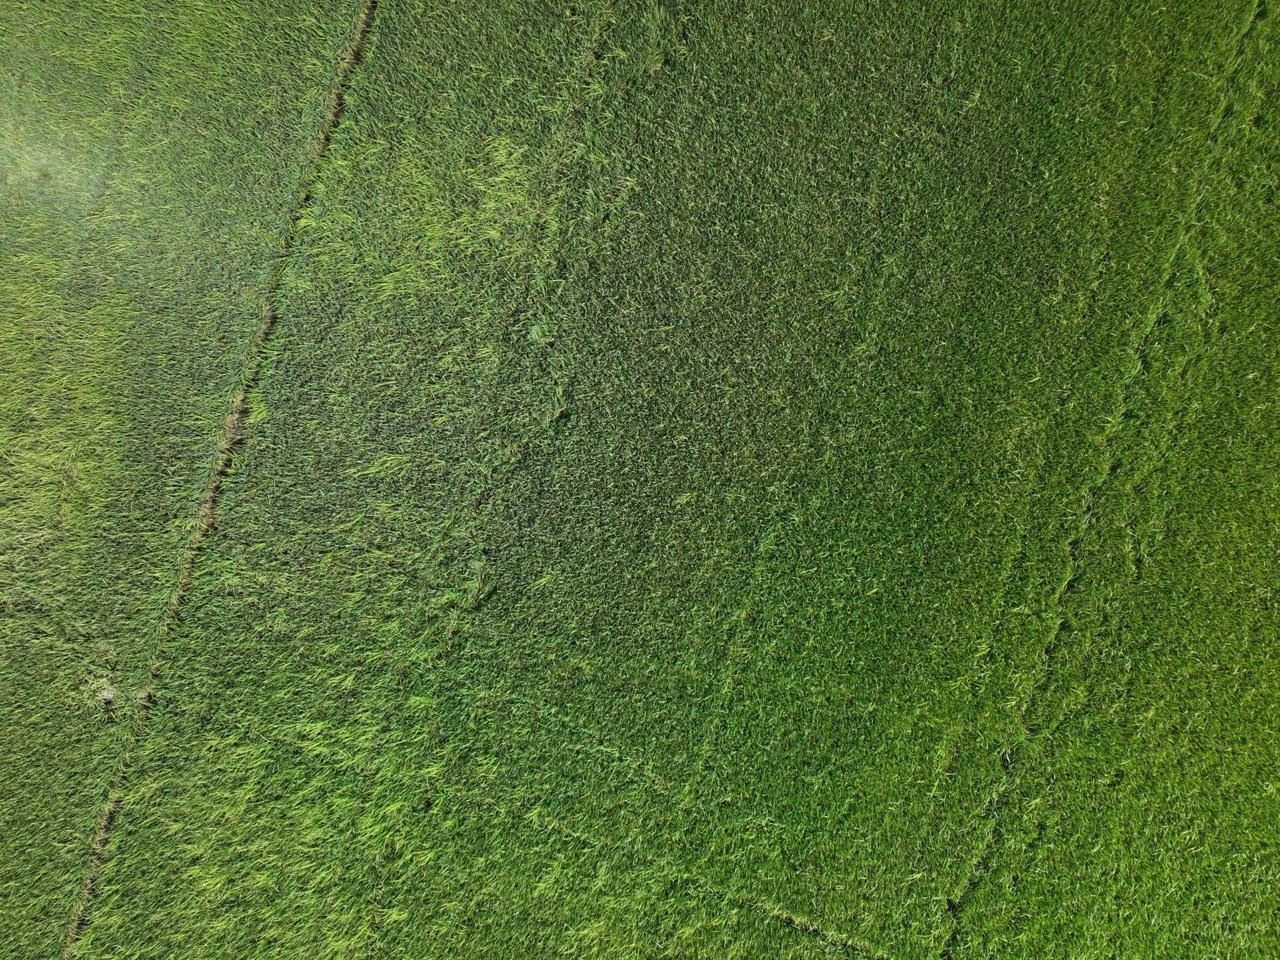
\includegraphics[width=10cm]{Images/sample.JPG}
    \caption{Sample of RGB field image from the dataset showing the visual similarity and overlap between crops and weeds, highlighting the importance of accurate crop-weed segmentation in precision agriculture.}
    \label{fig:sample}
\end{figure}
The global population is growing at an unprecedented rate and is estimated to reach nearly 9 billion by 2050, resulting in a significantly increased demand for food, feed, fiber, and fuel. This situation creates the need for a substantial increase in agricultural productivity \cite{fao2017future}. However, modern agriculture faces many challenges, including decreasing arable land, climate change, and the growing problem of weeds. As a result, significant losses occur in crop production, and weeds can reduce the productivity of crops by 25\%. This means effective weed management is an important component of sustainable agriculture. This problem becomes more serious in rice fields as weedy rice is morphologically very similar to conventionally cultivated rice during the early growth stages, making it difficult to distinguish. As illustrated in Fig.~\ref{fig:sample}, even visual inspection of field images often makes it challenging to clearly distinguish crops from weeds due to overlapping vegetation, similar texture, and comparable color appearance. This morphological similarity makes visual identification difficult and labor-intensive, which often results in delays in intervention or reduced effectiveness\cite{weedy_rice_review}\cite{shahi2023weed}. Conventional weed management methods, such as manual inspection and uniform herbicide spraying, are not only inefficient but also unsustainable from an environmental perspective due to increased chemical usage.



To tackle these issues, precision agriculture is increasingly using unmanned aerial vehicles (UAVs) alongside deep learning methods for the automated differentiation of crops and weeds. Imaging via UAVs allows for the capture of high-resolution images of agricultural fields, offering detailed spatial data crucial for identifying weeds at an early stage \cite{zhao2025deep,saini2025review,pena2013weedmapping,sa2018weednet,bah2018weed,fan2023crossmodal_weed}. In this context, models based on Convolutional Neural Networks (CNNs), including \textit{YOLO}\cite{yaseen2025yolov8}, \textit{Mask R-CNN} \cite{he2017maskrcnn}, \textit{U-Net}\cite{ronneberger2015unet}, \textit{SegNet} \cite{badrinarayanan2017segnet}, and \textit{DeepLab}\cite{chen2017deeplabv3}\cite{chen2018Deeplabv3plus}, have shown excellent results in tasks involving semantic segmentation. For instance, Silva et al. \cite{silva2024deep} presented a comparison among different variants of YOLO, U-Net, and Mask R-CNN, where YOLOv8s achieved more than 99.7\% precision on publicly available aerial images of soybeans and beans.

CNNs have demonstrated good performance in segmentation tasks by exploiting local spatial features, but they still face challenges in complex scenarios, such as agricultural crop-weed segmentation. This is because they cannot effectively model the long-range contextual dependencies that are crucial in complex agricultural scenes. To address this challenge, attention-based approaches, such as the Convolutional Block Attention Module (CBAM), have emerged as effective solutions \cite{woo2018cbam,hu2018senet,oktay2018attentionunet,wang2018nonlocal}. These mechanisms allow the models to learn long-range dependencies and improve the extraction of global contextual information. For instance, Li et al.\cite{li2025improved} have shown 3.08\% improvement on  UNet architecture by leveraging attention mechanisms on the sugar beet dataset. Besides, Transformer-based methods  \cite{dosovitskiy2021vit, xie2021segformer, liu2021swin} are proposed to further improve the modeling of global context. However, the application of these methods in real-time UAV-based applications is still hampered by two main limitations, namely, the requirement of large-scale training datasets and the high computational complexity. For instance, Jiang et al.\cite{jiang2022transformer} explore different variants of transformer on their in-house weed datasets and report that SegFormer achieves the best mIoU 65.74\% compared to all other variants, ie Swin Transformer.
Another important trend in crop–weed segmentation is the fusion of vegetation indices \cite{hunt2013vegetation} and multispectral imaging \cite{zhang2021multispectral} with RGB data. Multispectral images provide additional spectral information about plant physiology, while vegetation indices characterize features such as chlorophyll content and vegetation vigor that are important for enhancing the separability of crops from weeds. Ma et al. \cite{ma2024vegetation_dl} have shown that the integration of these modalities into deep learning frameworks could improve the segmentation performance. However, most existing methods use simple early fusion strategies, which cannot effectively solve the distribution shift problem from heterogeneous data modalities. 


Existing approaches offer distinct advantages and also have certain limitations in segmenting weedy rice under challenging field conditions. CNN encoder-decoders such as U-Net and DeepLabV3 capture local texture and multi-scale context through atrous convolution, but their receptive fields are limited, and reasoning across overlapping plants is difficult. Attention modules such as CBAM can adjust the channel and spatial locations at a low cost, but can not enhance the features extracted by the backbone. Transformer-based models can capture global context but require large annotated datasets and heavy computation, which is unaffordable for small UAV datasets and field deployment. Multispectral bands and vegetation indices can add physiological cues that RGB lacks \cite{ma2024vegetation_dl}, but they are usually combined with RGB by stacking channels at the input \cite{li2022attention_agriculture,yang2025rshrnet}. This may force one set of early filters to model modalities with different statistics. There is no single approach that addresses all these limitations.



Hence, we propose \textbf{$\mathbf{M^2}$FA-Net}, a Multi-Level Multimodal Fusion framework for crop-weed segmentation.
The proposed method performs hierarchical feature fusion at multiple progressive encoder levels, enabling the model to capture complementary cross-modal cues at multiple spatial resolutions and
abstraction levels. CBAM attention modules are applied after each fusion level to selectively recalibrate the integrated
features. Deep supervision via auxiliary classifiers provides rich intermediate gradient signals, and a composite loss
function jointly optimizes pixel accuracy, region overlap, and boundary sharpness. Specifically, features from two modality-specific encoders are fused at each of the four encoder stages using concatenation followed by a learned $1\times1$ convolution, while each input modality is evaluated separately.

Although individual blocks are well established, the novelty of $M^2$FA-Net lies in its integration, which differentiates it from existing RGB-multispectral approaches in 3 key aspects.
\begin{enumerate}
    \item\textit{Fusion location:} Two modality-specific encoders are fused at every encoder stage rather than at the input or at a single late stage. 
    \item \textit{Information interaction:} At each stage, concatenated features are combined by a learnable $1\times1$ convolution and then refined through CBAM, enabling interaction between the modalities at every scale. 
    \item \textit{Feature selection:} CBAM utilizes channel attention to assign different weights to RGB, multispectral, and vegetation indices, while spatial attention identifies the most informative regions. Auxiliary classifiers are applied to intermediate fused features that provide direct gradient feedback to each fusion stage.
\end{enumerate}



The main contributions of this work are summarized as follows:
\begin{itemize}
\item Proposed a dual-stream DeeplabV3 architecture pretrained on ResNet50 that fuses RGB and multispectral features at multiple hierarchical encoder levels, enabling adaptive integration of complementary cross-modal information across all spatial resolutions.
\item Integrated CBAM attention modules at each fusion stage to selectively emphasize discriminative channel and spatial features, suppressing background noise and improving cross-modal feature quality at every level of abstraction.
\item Introduced a deep supervision mechanism via multiple auxiliary segmentation classifiers attached to intermediate fusion stages, providing dense gradient flow to all backbone layers and substantially improving convergence and final segmentation performance. 
\item Adopted a composite loss function that combines cross-entropy, Dice, and boundary-sensitive loss terms, jointly optimizing pixel-level accuracy, region overlap, and boundary sharpness for challenging crop-weed segmentation.
\item Experimented on the WeedyRice-RGBMS-DB dataset and achieved best performance among the evaluated methods, with a test IoU of 80.79\% and a Dice score of 89.21\%, surpassing eleven competitive baseline models.
\item Conducted an input-modality study to quantify the contributions of multispectral bands and individual vegetation indices to the model performance.

% Systematic ablation studies validate the contribution of each component.
\end{itemize}
\section{Related Works}
Agricultural image analysis has made remarkable progress with the rise of deep learning, enhancing crop monitoring, disease diagnosis, weed detection, and semantic segmentation tasks significantly \cite{lei2024segmentationreview}. We are moving away from handcrafted feature-based methods that have been widely used in previous studies, as such approaches often fail in real-world conditions with illumination variation, occlusion, and complex backgrounds. Weed detection and segmentation remain particularly challenging tasks due to the visual similarities between crops and weeds, varying lighting conditions, and different soil backgrounds \cite{zhao2025deep,saini2025review}. Over time, researchers have explored a wide spectrum of strategies, ranging from convolutional networks to attention-enhanced models and transformer-based frameworks, as well as multimodal data fusion using both RGB and multispectral images, enabling the extraction of vegetation indices such as NDVI and NDRE.

\subsection{CNN-Based Segmentation Approaches}
Convolutional Neural Networks laid the foundation of semantic segmentation in precision agriculture. Encoder-decoder architectures such as U-Net \cite{ronneberger2015unet}, U-Net++ \cite{zhou2018unet++}, PSPNet \cite{zhao2017pyramid}, HRNet \cite{sun2019high}, DenseUNet \cite{safarov2021denseunet}, and DeepLabV3+ \cite{chen2018Deeplabv3plus} have been widely adopted for UAV-based crop monitoring and weed mapping, demonstrating strong ability to capture local spatial patterns and contextual scene information \cite{silva2024deep}. Among these, DeepLabV3+ has drawn attention for its use of atrous convolutions and Atrous Spatial Pyramid Pooling (ASPP), which increase the receptive field with minimal extra computation, making it suitable for dense prediction tasks like weed segmentation\cite{chen2018Deeplabv3plus}. To further improve performance, attention mechanisms such as the Convolutional Block Attention Module (CBAM)\cite{woo2018cbam} have been introduced into CNN pipelines, jointly modeling channel and spatial attention to improve localization accuracy and boundary precision in agricultural scenes\cite{li2022attention_agriculture}. Beyond architectural choices, boundary-aware loss functions and deep supervision strategies have also proven effective in producing improved segmentation outputs, especially where precise plant contour delineation matters for targeted herbicide application. 


Recent studies have also explored lightweight deep learning
models for weed identification on resource-constrained
devices. Li et al. \cite{li2026wagenet} proposed WAGENet,
a hardware-aware lightweight network for weed
classification on low-power microcontrollers.
Zhang et al. \cite{zhang2026tinymlkd} introduced a
TinyML-enabled IoT framework that employs knowledge
distillation to improve the efficiency of on-device
weed classification. Similarly, Zhang et al.
\cite{zhang2026tinyweednet} developed TinyWeedNet,
a hardware-efficient CNN for real-time weed
identification on embedded devices. These studies
demonstrate the importance of computational efficiency
for practical agricultural applications. However,
they primarily address image-level weed classification,
whereas the present work focuses on pixel-level
segmentation using multimodal RGB and multispectral
imagery.



\subsection{Transformer-Based Segmentation Approaches}
More recently, transformer-based models have been introduced in the field of agricultural segmentation, which provide a completely different paradigm through global self-attention mechanisms.
Architectures such as Vision Transformer (ViT)
\cite{dosovitskiy2021vit}, SegFormer
\cite{xie2021segformer}, Segmenter
\cite{strudel2021segmenter}, and Swin Transformer
\cite{liu2021swin} build on the transformer
architecture introduced by Vaswani et al.
\cite{vaswani2017attention}. These have achieved powerful segmentation performance by capturing long-range spatial dependencies that CNNs find intrinsically difficult to capture. This global context awareness is especially helpful in cluttered agricultural scenes where local features alone may not be sufficient to distinguish visually similar plant species. Besides supervised learning paradigms, alternative learning methods for agricultural vision tasks have also been explored in recent research. Kumar et al. \cite{kumar2024zeroshot} proposed a semantic attribute-based zero-shot learning framework for plant disease classification and proved that attribute-guided representations could improve the recognition of unseen disease categories. Such approaches are indicative of the growing curiosity in developing more data-efficient learning methods for agricultural applications. However, a major limitation of pure transformer models is their heavy dependence on large annotated datasets and their high computational requirements, which are practical barriers to real-time deployment in field-based agricultural systems.
\subsection{Hybrid and Multimodal Fusion Approaches}
Recognizing that CNNs and transformers have complementary strengths, hybrid frameworks have been proposed to combine both of these architectures so that local feature extraction and global contextual modeling can be done together and yield improved segmentation robustness \cite{zhou2018unet++}. Alongside architectural hybridization, multimodal data fusion has emerged as another direction. RGB imagery alone often falls short under challenging conditions such as changing illumination and background conditions, prompting researchers to integrate multispectral bands - particularly Near Infrared (NIR) and Red Edge (RE) — highly correlated with plant physiology \cite{zhang2021multispectral}. Sahin et al. \cite{sahin2023segmentation} fused RGB and multispectral inputs within a CRF-enhanced U-Net framework and reported meaningful segmentation gains on sunflower weed datasets, while Ma et al. \cite{ma2024vegetation_dl} showed that adding vegetation indices to multispectral data improves robustness under different field conditions. Although early concatenation remains a common
fusion strategy \cite{li2022attention_agriculture,
yang2025rshrnet}, recent studies have explored
attention-based and multi-scale cross-modal fusion
to better integrate heterogeneous spatial and
spectral information. 
Recent studies have investigated advanced multimodal
fusion strategies for agricultural segmentation and
remote sensing. Fan et al. \cite{fan2024cmfnet} proposed CMFNet,
which integrates RGB and near-infrared imagery through
cross-modal feature interaction and attention-based
refinement for field weed mapping. Dong et al. \cite{dong2026asvlb}
introduced ASVLB-Net, employing NDVI-guided adaptive
fusion for multispectral weed segmentation. Similarly,
SCG-UNet\cite{li2026scgunet} combines UAV RGB and multispectral
imagery using channel-spatial feature enhancement and
attention-guided skip connections for soybean weed
segmentation. In remote sensing, Cross Mamba Fusion
Network\cite{cmfnet2025mamba} employs Cross-Mamba modules to integrate
hyperspectral and LiDAR features for classification.

Although these methods demonstrate the effectiveness
of multimodal feature integration, they differ in
their fusion architectures, input modalities, and
learning objectives. The proposed $M^2$FA-Net
employs independent RGB and multispectral encoders
with hierarchical feature fusion at four encoder
stages. At each stage, concatenated features are
integrated through a learnable $1\times1$ convolution
and refined using CBAM, while deep supervision
supports intermediate feature learning.
Table~\ref{tab:fusion_comparison} summarizes the
architectural differences between these approaches
and the proposed framework.


\begin{table*}[t]

\centering
\small
\setlength{\tabcolsep}{4pt}
\renewcommand{\arraystretch}{1.3}

\caption{Comparison of recent multimodal fusion approaches
for agricultural segmentation and remote sensing.}
\label{tab:fusion_comparison}

\begin{tabular}{p{0.17\textwidth}
                p{0.17\textwidth}
                p{0.28\textwidth}
                p{0.28\textwidth}}
\hline
\textbf{Method} &
\textbf{Input Modalities} &
\textbf{Fusion Strategy} &
\textbf{Architectural Characteristics} \\
\hline

CMFNet (2024)\cite{fan2024cmfnet}
& RGB + NIR
& Cross-modal multi-scale feature fusion
& Cross-modal enhancement and attention-based
feature refinement for weed segmentation \\

\hline

Cross Mamba Fusion Network (2025)\cite{cmfnet2025mamba}
& Hyperspectral + LiDAR
& Global--local feature extraction with
Cross-Mamba fusion
& Mamba-based multimodal interaction for
remote-sensing classification \\

\hline

ASVLB-Net (2026)\cite{dong2026asvlb}
& Multispectral + NDVI
& NDVI-guided adaptive feature fusion
& Lightweight architecture for spectral
and vegetation feature integration \\

\hline

SCG-UNet (2026)\cite{li2026scgunet}
& RGB + Multispectral
& Channel--spatial attention and
attention-guided skip fusion
& U-Net-based architecture for
weed segmentation \\

\hline

\textbf{$M^2$FA-Net (Proposed)}
& \textbf{RGB + Multispectral + NDVI/NDRE}
& \textbf{Four-stage hierarchical fusion
with $1\times1$ convolution and CBAM}
& \textbf{Independent modality encoders,
progressive fusion, and deep supervision} \\

\hline
\end{tabular}
\end{table*}
Although recent studies have reported improved crop-weed segmentation performance using modified encoder-decoder and ensemble architectures \cite{ganapathy2025cropweed}, most approaches remain dependent on RGB imagery and do not fully exploit complementary multispectral information. Despite progress in these areas, several challenges remain unresolved. Most CNN-based algorithms rely only on RGB imagery and do not benefit from the full range of spectral information available with multispectral sensors. Transformer-based approaches, while powerful in modeling global context, demand substantial annotated data and computational resources that are often impractical in real agricultural deployment scenarios. Hybrid fusion methods have made strides in combining spatial and spectral modalities, yet they predominantly employ simplistic early fusion strategies that fail to capture the complementary nature of heterogeneous data streams at multiple representational levels. Furthermore, relatively few studies have brought together vegetation indices, hierarchical multimodal feature fusion, lightweight attention mechanisms, deep supervision, and boundary-aware optimization within a single cohesive segmentation framework. These collective gaps motivate the present work, which proposes a multi-level fusion DeepLab-based architecture integrating dual-stream ResNet50 backbones, CBAM attention, and a composite loss function designed to deliver accurate and robust weed segmentation under complex, real-world agricultural conditions.

\begin{figure*}[t]
\centering
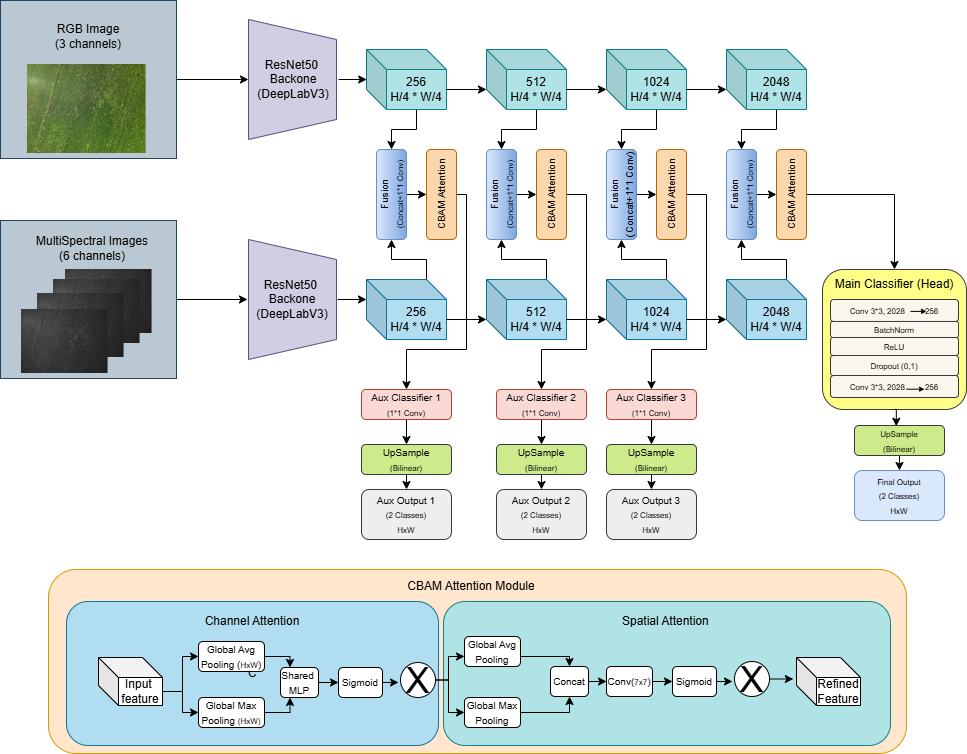
\includegraphics[width=\linewidth]{Images/MNet_architecture.png}
\caption{Architecture of the proposed $M^2$FA-Net for multimodal weed segmentation.}
\label{fig:mnet_architecture}
\end{figure*}
\section{Methodology}
% \subsection{Overview}
In this work, we propose $M^2$FA-Net, a multimodal attention-driven semantic segmentation framework for accurate weed segmentation using RGB and multispectral imagery. Figure~\ref{fig:mnet_architecture} shows the proposed architecture and it combines spatial information from RGB images with spectral and vegetation-specific information extracted from multispectral bands and vegetation indices. The overall architecture consists of two parallel DeepLabV3-ResNet50 backbone networks: one processes RGB images while the other processes multispectral inputs containing spectral bands and vegetation indices. Unlike conventional late-fusion approaches that combine modality-specific representations only at the final encoder stage, the proposed method fuses feature maps extracted at different semantic levels progressively using concatenation and 1 × 1 convolution operations, enabling the integration of complementary spectral-spatial cues at every scale of abstraction. At each fusion level, a CBAM attention module recalibrates the fused representation\cite{hu2018senet,wang2018nonlocal}. The final fused representation is passed through a segmentation head to generate dense pixel-wise weed predictions. Additionally, deep supervision and a composite loss function are incorporated to improve optimization stability, gradient flow, and segmentation boundary quality \cite{lee2015dsn}.

\subsection{Input Modalities}
Our framework considers two primary complementary input modalities:
\begin{itemize}
    \item \textbf{RGB Images:} Standard three-channel RGB images that capture spatial structures, texture patterns, and color information.
    \item \textbf{Multispectral Data:} Four spectral bands, namely Green (G), Red (R), Red Edge (RE), and Near-Infrared (NIR), which provide important spectral and physiological information related to vegetation characteristics.
\end{itemize}
To further improve crop-weed discrimination, two vegetation indices are computed from the multispectral bands.
\subsubsection{Normalized Difference Vegetation Index (NDVI)}
NDVI is expressed in the equation ~\ref{eq1}.
\begin{equation}
\text{NDVI} = \frac{NIR - R}{NIR + R}\label{eq1}
\end{equation}
NDVI \cite{rouse1974ndvi} highlights vegetation health by exploiting the strong reflectance of healthy vegetation in the NIR spectrum and absorption in the red spectrum.
\subsubsection{Normalized Difference Red Edge Index (NDRE)}
NDRE is defined in the equation ~\ref{eq2}.
\begin{equation}
\text{NDRE} = \frac{NIR - RE}{NIR + RE}\label{eq2}
\end{equation}
NDRE \cite{gitelson1997chlorophyll} is more sensitive to chlorophyll concentration and plant stress, making it highly effective for precision agriculture applications. Consequently, the multispectral representation is extended into a six-channel input consisting of \{G, R, RE, NIR, NDVI, NDRE\}. Per-channel mean and standard deviation statistics are computed over the training set and used to normalize the multispectral input using Z-scores. This multimodal representation provides complementary spatial, spectral, and vegetation-specific information for robust weed segmentation.

\subsection{Network Architecture}
$M^2$FA-Net adopts a dual-stream multi-level fusion strategy based on DeepLabV3 with ResNet50 backbones. The architecture is specifically designed to preserve modality-specific characteristics while reliably integrating spatial and spectral information.


\subsubsection{Dual-Stream Multi-Level Feature Extraction and Fusion}
We employ two independent DeepLabV3-ResNet50 encoders pretrained on the COCO-with-VOC-labels benchmark: an RGB encoder for three-channel RGB image, and a multispectral encoder for six-channel multispectral input comprising spectral bands and vegetation indices. As DeepLabV3 is originally designed for three channel input, the RGB encoder retains its original architecture, processes the three channel input without modification, while the first convolutional layer of the multispectral encoder is modified to accept six input channels. For the main experiments, the first three
multispectral input channels inherit the
corresponding pretrained RGB convolutional
weights, while the remaining three channels
are initialized using their channel-wise mean.
In the separate input-modality experiments,
all multispectral input channels are initialized
using the mean pretrained RGB weights.

At each of the four encoder stages $i=1,\dots,4$, the encoder outputs feature maps with progressively increasing channel dimensions and decreasing spatial resolutions, capturing the information at different semantic levels: low-level features represents edges, textures, and local structures; mid-level features represents plant structures and shape information; and high-level features capture semantic representations relevant to crops and weed identification. The extracted feature maps from the RGB and multispectral branches are stored independently for subsequent hierarchical fusion. Unlike the traditional late fusion approaches that integrates modalities at the final layers, the proposed approach performs fusion at every encoder stage to extract complementary information across multiple feature levels. This helps the model to utilize cross-modal interactions through out the feature levels. At each encoder stage, the RGB and multispectral feature maps are combined along the channel dimension and is expressed in the equation~\ref{eq3}. 
\begin{equation}
F_{fusion}^{(i)} = \text{Concat}(F_{rgb}^{(i)}, F_{ms}^{(i)})\label{eq3}
\end{equation}
where $F_{rgb}^{(i)}$ and $F_{ms}^{(i)}$ are RGB and multispectral features at the $i^{th}$ encoder level, respectively. After concatenation, a $1\times1$ convolution is applied to reduce dimensionality and learn optimal feature interactions:
\begin{equation}
F_{reduced}^{(i)} = \text{Conv}_{1\times1}(F_{fusion}^{(i)})
\end{equation}
This step integrates diverse spatial and spectral features without increasing the network's channel depth \cite{lin2017fpn}.


\subsubsection{CBAM Attention Module}

To enhance feature representation further, the Convolutional
Block Attention Module (CBAM)~\cite{woo2018cbam} is applied
to the fused features at each level. CBAM sequentially applies
channel attention and spatial attention.

\paragraph{Channel Attention:}
This attention identifies the most informative feature
channels by learning inter-channel relationships and is
expressed by Eq.~\ref{eq5}.
\begin{equation}
F_{c}^{(i)} = M_c(F_{reduced}^{(i)}) \otimes
F_{reduced}^{(i)}
\label{eq5}
\end{equation}
where $M_c$ denotes channel attention and $\otimes$
represents element-wise multiplication.

\paragraph{Spatial Attention:}
This attention focuses on important spatial regions within
the feature map and is defined in Eq.~\ref{eq6}.
\begin{equation}
F_{s}^{(i)} = M_s(F_c^{(i)}) \otimes F_c^{(i)}
\label{eq6}
\end{equation}
where $M_s$ represents spatial attention.

The final attention-refined representation is given
in Eq.~\ref{eq8}.
\begin{equation}
F_{att}^{(i)} = F_s^{(i)}
= \operatorname{CBAM}(F_{reduced}^{(i)})
\label{eq8}
\end{equation}

The attention mechanism enables the network to suppress
irrelevant background information, such as soil and shadows,
while emphasizing discriminative weed regions.

\subsubsection{Deep Supervision}
To facilitate gradient flow and stabilize training, auxiliary classifiers are attached to intermediate feature levels. These auxiliary outputs provide additional supervision during training and encourage meaningful feature learning at different semantic scales. The $L_{\text{final}}$ is expressed in the equation ~\ref{eq9}
\begin{equation}
L_{\text{final}} = L_{\text{main}} + \lambda \sum_{l=1}^{N} L_{\text{aux}}^{l}\label{eq9}
\end{equation}
where \(L_{\text{main}}\) represents the primary segmentation loss computed from the final output prediction, while \(L_{\text{aux}}^{l}\) denotes the auxiliary losses obtained from intermediate supervision levels. The weighting factor \(\lambda\) controls the contribution of auxiliary losses, and \(N\) represents the total number of supervised intermediate levels in the multi-level architecture.
\subsubsection{Segmentation Head}
The last fused feature representation is passed through a segmentation head consisting of convolution, batch normalization, ReLU activation, and dropout layers. The final prediction layer generates pixel-wise logits corresponding to the weed and background classes. 
The low-resolution segmentation map is upsampled to the original image resolution using bilinear interpolation and expressed in equations ~\ref{eq10}~\ref{eq11}.

\begin{equation}
F_{\text{seg}} =
\operatorname{Conv}_{1\times1}
\left(
\operatorname{Conv}_{3\times3}
\left(F_{att}^{(4)}\right)
\right)
\label{eq10}
\end{equation}

\begin{equation}
F_{\text{out}} = Upsample(F_{\text{seg}})\label{eq11}
\end{equation}
where $F_{seg}$ represents the predicted segmentation map before upsampling.
\subsection{Loss Function}

The model is trained using a composite loss function combining three complementary terms to improve segmentation quality and boundary precision.

\subsubsection{Cross-Entropy Loss}

Cross-Entropy Loss supervises pixel-wise classification:

\begin{equation}
\mathcal{L}_{CE} = - \sum_{i} y_i \log(\hat{y}_i)
\label{eq:ce_loss}
\end{equation}

where $y_i$ and $\hat{y}_i$ represent ground truth and predicted probabilities, respectively.

\subsubsection{Dice Loss}

Dice Loss directly optimizes region overlap between predicted and ground-truth masks:

\begin{equation}
\mathcal{L}_{Dice} = 1 - \frac{2 \sum_{i=1}^{N} (p_i g_i) + \alpha}
{\sum_{i=1}^{N} p_i + \sum_{i=1}^{N} g_i + \alpha}
\label{eq:dice_loss}
\end{equation}

where $p_i$ denotes the predicted foreground probability for pixel $i$, $g_i$ represents the corresponding ground-truth binary value, $N$ indicates the total number of pixels, and $\alpha$ is a smoothing factor introduced to prevent division by zero \cite{milletari2016vnet}.
Dice Loss is specifically effective under the conditions of class imbalance, which is commonly observed in weed segmentation datasets.
\subsubsection{Boundary Loss}
To increase the contour sharpness and localization of the boundaries, we introduce a Boundary Loss based on Laplacian edge detection. 
\begin{equation}
E_{p} = \text{Conv}_{\text{Lap}}(P), \qquad
E_{g} = \text{Conv}_{\text{Lap}}(G)
\end{equation}
\begin{equation}
\mathcal{L}_{Boundary} = \frac{1}{N} \sum_{i=1}^{N} \left| E_{p}^{i} - E_{g}^{i} \right|
\label{eq:boundary_loss}
\end{equation}
where $P$ and $G$ denote the predicted segmentation map and ground truth mask, $E_p$ and $E_g$ represent their corresponding edge maps, and $N$ is the total number of pixels \cite{kervadec2019boundary}.
\subsubsection{Overall Loss}

The primary segmentation loss $\mathcal{L}_{\text{main}}$ is defined in the equation ~\ref{eq12}

\begin{equation}
\mathcal{L}_{main} =
0.4\mathcal{L}_{CE}
+
0.4\mathcal{L}_{Dice}
+
0.2\mathcal{L}_{Boundary}\label{eq12}
\end{equation}
The $\mathcal{L}_{main}$ enables the model to improve classification accuracy, region overlap, and boundary precision simultaneously.
\section{Experiments}
To make the comparisons fair, All models were implemented in PyTorch and evaluated on the WeedyRice-RGBMS-DB dataset
using the same training, validation, and
testing partitions, input resolution, and
evaluation metrics. Common preprocessing
and augmentation procedures were applied
to ensure consistent experimental conditions.
The training configuration of the proposed
framework is summarized in
Table~\ref{tab:training_details}. 
The training process for all models used both RGB and multispectral images, it was performed on a 13th Gen Intel(R) Core i9-13900K (3.00 GHz) processor, an NVIDIA RTX A5000 GPU with 24 GB memory, 128 GB RAM, 1 TB SSD, and 2 TB HDD. The Software environment was Windows 11 Pro, Python 3.10.20, and CUDA 12.4 for accelerated training. The detailed training hyperparameters and optimization settings are presented in Table~\ref{tab:training_details}. We conducted a series of experiments on the WeedyRice-RGBMS-DB based on a uniform training and testing scheme. Our algorithm is compared against other state-of-the-art models, such as CNN models (U-Net), transformer models (Vision Transformer and SegFormer), as well as the hybrid models (TransUNet, Swin models, and DeepLabV3+). To thoroughly investigate the proposed model, all methods are evaluated under the same conditions and fairly compared with the standard segmentation metrics, including Accuracy, Precision, Recall, IoU, and Dice coefficient. The results are given as the mean ± standard deviation over several runs to evaluate robustness. Moreover, ablation studies and qualitative comparisons were carried out to analyse the contribution of each component of our proposed model.
% \subsection{Training Strategy}
% $M^2$FA-Net framework is optimized using the AdamW optimizer \cite{loshchilov2019adamw} with weight decay regularization. A warmup cosine learning rate schedule \cite{loshchilov2017sgdr} is employed to stabilize early-stage optimization and improve convergence during later epochs. During the warmup phase, the learning rate gradually increases to the base learning rate. Subsequently, cosine annealing progressively reduces the learning rate to achieve smoother convergence. Mixed precision training is additionally employed to improve GPU memory efficiency and accelerate training. Data augmentation techniques, including horizontal flipping and vertical flipping, are also utilized to improve generalization capability under varying agricultural conditions. The detailed training hyperparameters and optimization settings are presented in Table~\ref{tab:training_details}.

\begin{table*}[t]
\centering
\caption{Training Details of the Proposed Framework}
\label{tab:training_details}
\resizebox{\textwidth}{!}{%
\renewcommand{\arraystretch}{1.1}
\setlength{\tabcolsep}{4pt}

\begin{tabular}{cccccccccccc}
\hline
Batch Size & Epochs & Optimizer & Initial LR & Min LR & Weight Decay & Warmup Epochs & Aux. Loss Weight ($\lambda$) & Dropout & Grad. Clip & Aug. Prob. & Input Resolution \\
\hline
8 & 20 & AdamW & $2\times10^{-4}$ & $1\times10^{-6}$ & $1\times10^{-3}$ & 3 & 0.7 & 0.1 & 1.0 & 0.5 & $512\times512$ \\
\hline

\end{tabular}
}
\end{table*}
\begin{table}[htbp]
\centering
\caption{Dataset Statistics and Split Details}
\label{tab:dataset_stats}
\begin{tabular}{|l|c|}
\hline
\textbf{Category} & \textbf{Count} \\ \hline

RGB Images & 734 \\ \hline
Segmentation Masks & 734 \\ \hline
Overlay Images & 734 \\ \hline
Multispectral Images (Total) & 2936 \\ \hline

\multicolumn{2}{|c|}{\textbf{Multispectral Breakdown (per RGB image)}} \\ \hline
Green (G) & 734 \\ \hline
Near-Infrared (NIR) & 734 \\ \hline
Red (R) & 734 \\ \hline
Red Edge (RE) & 734 \\ \hline

\multicolumn{2}{|c|}{\textbf{Dataset Split}} \\ \hline
Training Set & 438 \\ \hline
Validation Set & 148 \\ \hline
Testing Set & 148 \\ \hline

\end{tabular}

\end{table}

\begin{figure*}[t]
\centering
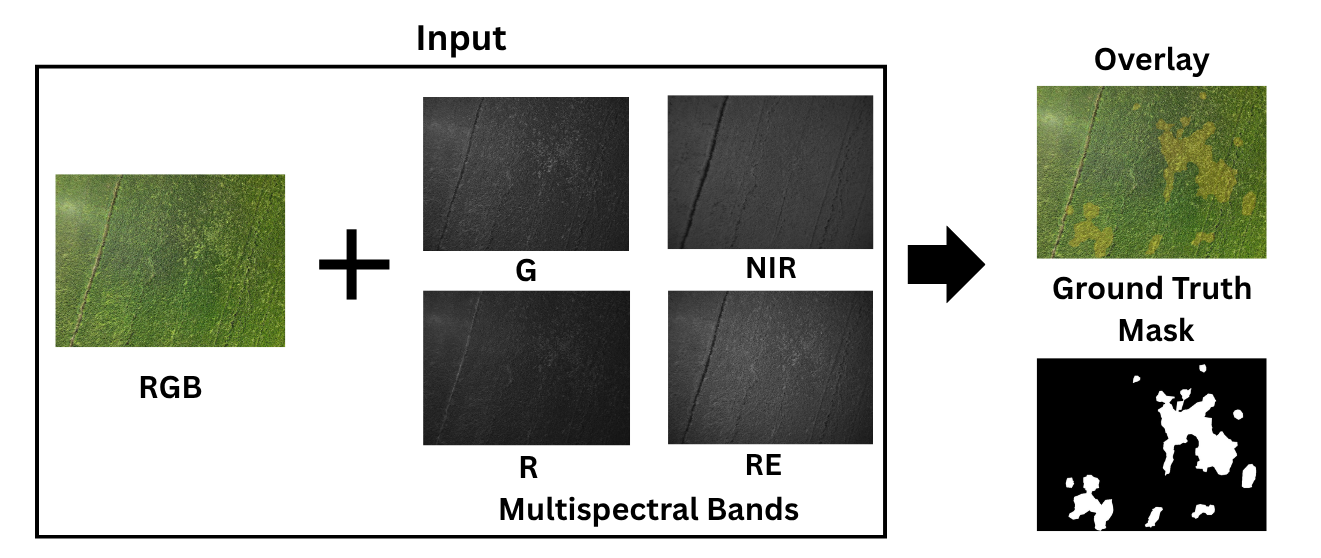
\includegraphics[width=\linewidth]{Images/Dataset_Sample3.png}
\caption{Overview of the WeedyRice-RGBMS-DB dataset structure. Each sample consists of an RGB image and corresponding multispectral bands, including Green (G), Near-Infrared (NIR), Red (R), and Red Edge (RE) channels. The dataset additionally provides overlay visualizations and pixel-wise ground truth masks for weed segmentation.}
\label{fig:dataset_sample}
\end{figure*}

\subsection{Dataset Description}
The experiments are conducted on the Weedy Rice RGB-Multispectral (WeedyRice-RGBMS-DB) dataset \cite{nguyen2025dataset}, a UAV-based multimodal dataset designed for weedy rice segmentation in agricultural fields. The dataset was collected using a DJI M3M UAV over rice fields in An Giang Province, Vietnam, and is geo-referenced in the WGS 84/UTM Zone 48N coordinate system. The imagery was acquired across three cropping seasons. We use the train:validation:test partition (438:148:148) supplied by the dataset authors without modification, so that our results are comparable under a common, publicly defined protocol. The public documentation does not specify the field, flight, or acquisition date of each sample, so we cannot exclude spatial adjacency or temporal continuity between partitions. According to the original dataset publication, the UAV flights were conducted with 70\% front and side image overlap to ensure sufficient spatial coverage. This percentage refers to overlap during image acquisition and does not indicate the degree of overlap between training and testing samples. Since the dataset documentation does not establish spatially independent partitions, potential correlation between neighboring images across the dataset splits cannot be ruled out. It includes RGB images, multispectral images, binary segmentation masks, overlay visualizations, and associated metadata. A sample dataset structure is shown in Fig~\ref{fig:dataset_sample}. The dataset consists of a total of 734 samples, divided into training, validation, and test splits. Each sample contains an RGB image (3 channels) along with multispectral bands, namely Green (G), Red (R), Red Edge (RE), and Near-Infrared (NIR), and a corresponding pixel-wise binary ground-truth mask. All images are resized to $512 \times 512$ resolution for uniform processing. For multispectral experiments, the model adopts a dual-stream architecture where the RGB encoder receives a 3-channel RGB image and the multispectral encoder receives a 6-channel input composed of 4 spectral bands and 2 vegetation indices.

In terms of dataset composition, the RGB subset contains 734 images of resolution $1280 \times 960$, while the multispectral subset includes 2936 spatially aligned band images (four bands per RGB image). The ground-truth masks (734 images) provide pixel-level annotations for weedy rice detection, where pixel value 255 denotes weedy rice and 0 represents the background. Overlay images are provided for qualitative evaluation. Metadata files include acquisition details such as GPS coordinates, altitude, timestamp, sensor type, and filename mappings to ensure data consistency. 
% \subsection{Experimental Setting}
% To make the comparisons fair, all the models are implemented in Pytorch and trained under identical experimental settings. The training process for all models used both RGB and multispectral images and was performed on a 13th Gen Intel(R) Core i9-13900K (3.00 GHz) processor, an NVIDIA RTX A5000 GPU with 24 GB memory, 128 GB RAM, 1 TB SSD, and 2 TB HDD. The Software environment was Windows 11 Pro, Python 3.10.20, and CUDA 12.4 for accelerated training. We used the same data split as in Table~\ref{tab:dataset_stats} for training, validation and testing. We considered all the evaluation metrics discussed in Section~\ref{evaluation_metrics} for the performance assessment.




\subsection{Evaluation Metrics}
\label{evaluation_metrics}

To quantify crop-weed segmentation result, performance is reported across five key metrics: Accuracy, Precision, Recall, IoU, and Dice score.
\begin{equation}
\text{Accuracy} = \frac{TP + TN}{TP + TN + FP + FN}
\label{eq:accuracy}
\end{equation}
\begin{equation}
\text{Precision} = \frac{TP}{TP + FP}
\label{eq:precision}
\end{equation}
\begin{equation}
\text{Recall} = \frac{TP}{TP + FN}
\label{eq:recall}
\end{equation}
\begin{equation}
\text{IoU} = \frac{TP}{TP + FP + FN}
\label{eq:iou}
\end{equation}
\begin{equation}
\text{Dice} = \frac{2TP}{2TP + FP + FN}
\label{eq:dice_metric}
\end{equation}
where $TP$, $TN$, $FP$, and $FN$ denote true positives, true negatives, false positives, and false negatives, respectively.


% \begin{table*}[t]
% \centering
% \caption{Comparison of the proposed method with CNN-based, transformer-based, and hybrid segmentation approaches. Results are reported as mean $\pm$ standard deviation (in \%).}
% \label{tab:comparison}
% \begin{tabular}{lccccc}
% \hline
% \textbf{Method} & \textbf{Accuracy (\%)} & \textbf{Precision (\%)} & \textbf{Recall (\%)} & \textbf{IoU (\%)} & \textbf{Dice (\%)} \\
% \hline

% \textbf{CNN-based} \\

% U-Net \cite{ronneberger2015unet} 
% & 84.17 $\pm$ 0.40 
% & 69.28 $\pm$ 0.54 
% & 76.54 $\pm$ 1.94 
% & 56.46 $\pm$ 1.28 
% & 69.98 $\pm$ 1.20 \\

% \hline
% \textbf{Transformer-based} \\

% Vision Transformer (ViT) \cite{dosovitskiy2021vit} 
% & 83.84 $\pm$ 0.25 
% & 65.03 $\pm$ 0.99 
% & 74.33 $\pm$ 1.30 
% & 54.43 $\pm$ 0.23 
% & 68.32 $\pm$ 0.23 \\

% SegFormer \cite{xie2021segformer} 
% & 87.73 $\pm$ 0.11 
% & 74.47 $\pm$ 1.04 
% & 71.58 $\pm$ 0.72 
% & 58.45 $\pm$ 0.33 
% & 71.74 $\pm$ 0.41 \\

% \hline
% \textbf{Hybrid (CNN + Transformer)} \\

% TransUNet \cite{chen2021transunet} 
% & 88.36 $\pm$ 0.52 
% & 74.39 $\pm$ 1.81 
% & 80.59 $\pm$ 1.53 
% & 63.55 $\pm$ 0.65 
% & 76.30 $\pm$ 0.55 \\

% Swin-UNet (Hybrid Swin Transformer) \cite{liu2021swin} 
% & 88.35 $\pm$ 0.16 
% & 76.92 $\pm$ 0.39 
% & 75.92 $\pm$ 1.41 
% & 62.16 $\pm$ 0.80 
% & 75.11 $\pm$ 0.74 \\

% CNN + Transformer + Contrastive \cite{chen2020simple} 
% & 89.95 $\pm$ 0.27 
% & 77.10 $\pm$ 1.20 
% & 83.01 $\pm$ 1.18 
% & 67.28 $\pm$ 0.49 
% & 79.37 $\pm$ 0.38 \\

% \hline
% \textbf{CNN (Advanced Baseline)} \\

% DeepLabV3+ \cite{chen2018deeplab} 
% & 90.83 $\pm$ 0.22 
% & 79.12 $\pm$ 1.37 
% & 82.24 $\pm$ 2.06 
% & 68.45 $\pm$ 0.31 
% & 80.22 $\pm$ 0.30 \\

% \hline
% \textbf{Proposed Method} \\

% \textbf{MAViF-Net} 
% & \textbf{91.33 $\pm$ 0.07} 
% & \textbf{80.63 $\pm$ 1.19} 
% & \textbf{83.10 $\pm$ 1.32} 
% & \textbf{70.00 $\pm$ 0.14} 
% & \textbf{81.46 $\pm$ 0.11} \\

% \hline
% \end{tabular}
% \end{table*}

% \subsection{Quantitative Results}

% All competing methods are re-implemented and trained under the same experimental settings, including identical data splits, input resolution, optimizer, and training schedule, to ensure a fair comparison. 

% \subsection{Experimental Protocol}

% Each experiment is repeated five times with different random seeds to ensure robustness and statistical reliability. The final performance is reported on the test set as mean $\pm$ standard deviation.


% \subsection{Comparison with State-of-the-Art Methods}

% To show the effectiveness of our proposed framework, we conducted extensive experiments and comparisons with a diverse set of state-of-the-art (SOTA) segmentation models. These comparative models covering CNN-based architectures, pure transformer-based models, and hybrid CNN-Transformer frameworks. The compared  methods include U-Net \cite{ronneberger2015unet}, Vision Transformer (ViT) \cite{dosovitskiy2021vit}, SegFormer \cite{xie2021segformer}, TransUNet \cite{chen2021transunet}, Swin Transformer-based architectures \cite{liu2021swin}, and DeepLabV3+ \cite{chen2018deeplab}. Further recent hybrid strategies incorporating contrastive learning and multimodal feature integration are included for comparison.

% The quantitative results in terms of Dice Score, Intersection over Union (IoU), Recall, Precision, Accuracy are reported in Table ~\ref{tab:comparison}. All the results are presented as mean $\pm$ standard deviation over five runs. The results reported in the table clearly show that the performance of the models improves as the representation capability and complexity of the model increases from CNN based to transformer-based and finally to hybrid based.

% Simple CNN-based architecture such as U-Net is a strong baseline model for segmentation kind of tasks. However, its receptive filed limits their capability to capture long-range dependencies in complicated agriculture environment, resulting lower IoU and Dice scores compared to advance models architectures.

% As Transformer-based models such as ViT and SegFormer consider self-attention mechanism, they are capable of capturing long-range dependency. However, still faces challenges in local information, which is crucial for discriminating crop-weed segmentation tasks, resulting degradation in performance. The segFromer's performance is somewhat good compared to ViT as it is specifically designed for segmentation tasks. While segFormers performance improves over U-Net in term of accuracy Precision, IoU, and Dice score, but their performance is underperformed compared  to hybrid( CNN+Transformers) based architectures.

% Hybrid based models such as TransUNet, and Swin-UNet overcome these challenges by combining both convolutions layers and transformer blocks for preserving both local and global dependencies. This combined model lead to significant improvement in Dice, IoU, Recall, Precision, Accuracy. Further we observed improvement in performance by integrating contrastive loss to these hybrid models. Integrating contrastive loss ensures the better discrimination in embedding space and  gives complementary information which is very useful in scenarios with overlapping vegetation and complicated environment, resulting improvement in all the performance measures.

% Compared to all other SoTA approaches, our proposed framework outperforms in term of all the performance measures. More specifically, The proposed framework achieves 70.00\% IoU and 81.46\% Dice score, outperforming the advanced baseline DeepLabV3+ by 2.26\% and 1.54\%, respectively. Even though the improvement is numerically moderate, but consistent across all the performance measures, and is also supported by low SD, highlighting stable performance across different run.

% It can be seen that the proposed algorithm gives the maximum value of recall (83.12), which is an indication of its efficiency in minimizing false negatives. This is especially critical for agriculture weed segmentation because missed regions in the weeds could affect future decisions. Though the precision is slightly inferior to that of DeepLabV3+, the combined effect of precision and recall produces better results in terms of image segmentation measures, such as Intersection-over-Union (IoU) and Dice score.

% In conclusion, these findings demonstrate that the proposed framework successfully leverages the capability of CNNs to maintain local features, the attention mechanism to maintain global information, and the use of multiple models and late fusion techniques for better differentiation of features.
\section{Results and Discussion}
To evaluate the effectiveness of the proposed framework, extensive experiments are conducted against a diverse set of state-of-the-art (SOTA) models, including CNN-based, transformer-based, and hybrid CNN--Transformer architectures. The compared methods include U-Net \cite{ronneberger2015unet}, PSPNet \cite{zhao2017pyramid}, U-Net++ \cite{zhou2018unet++}, DenseUNet \cite{mu2023densenet}, DeepLabV3 \cite{chen2018Deeplabv3plus}, Vision Transformer (ViT) \cite{dosovitskiy2021vit}, SegFormer \cite{xie2021segformer}, Swin Transformer-based models \cite{liu2021swin}, CRF-UNet \cite{sahin2023segmentation}, and hybrid CNN-Transformer, frameworks \cite{guo2025cnn_transformer}.

Table~\ref{tab:results} presents the quantitative results, where all metrics are reported as mean $\pm$ standard deviation (in \%) over five independent runs, each with a different seed value. The results show a gradual performance improvement from conventional CNN-based methods to transformer-based and hybrid architectures, highlighting the importance of adaptively combining local spatial information with global contextual representations.

CNN-based architectures such as U-Net provide a strong baseline, achieving 89.68\% accuracy and a 68.75\% IoU. These models capture local spatial patterns important for distinguishing crop and weed textures. However, their receptive field is limited, which restricts their ability to model long-range contextual dependencies in complex agricultural scenes. Advanced CNN architectures attempt to address this limitation through improved feature aggregation strategies. PSPNet learns the context information of multiple scales by pyramid pooling, U-Net++ improves the feature propagation by nested skip connections, and DenseUNet applies dense connectivity to reuse features more effectively. Thus, DenseUNet achieves better performance than other conventional CNN-based methods with an IoU score of 70.67\%, while U-Net++ also provides competitive performance through improved feature propagation.

Transformer-based approaches such as ViT and SegFormer use self-attention mechanisms to better capture global dependencies. However, the local inductive bias of pure transformer architectures is weaker, which limits their ability to preserve the fine spatial details needed for accurate boundary localization. As a result, ViT achieves only 56.08\% IoU, while SegFormer improves the performance to 59.04\% IoU and 73.13\% Dice through hierarchical feature representations. Nevertheless, these models still underperform compared to stronger CNN-based approaches such as DenseUNet. Hybrid CNN-Transformer architectures combine the strengths of both paradigms by jointly learning local texture information and global contextual relationships. This leads to improved segmentation performance, with CNN+Transformer and Swin Transformer achieving IoU scores of 63.55\% and 75.43\%, respectively. However, their performance remains limited due to insufficient exploitation of multimodal spectral information and the absence of effective feature fusion mechanisms.
\begin{figure*}[t]
\centering
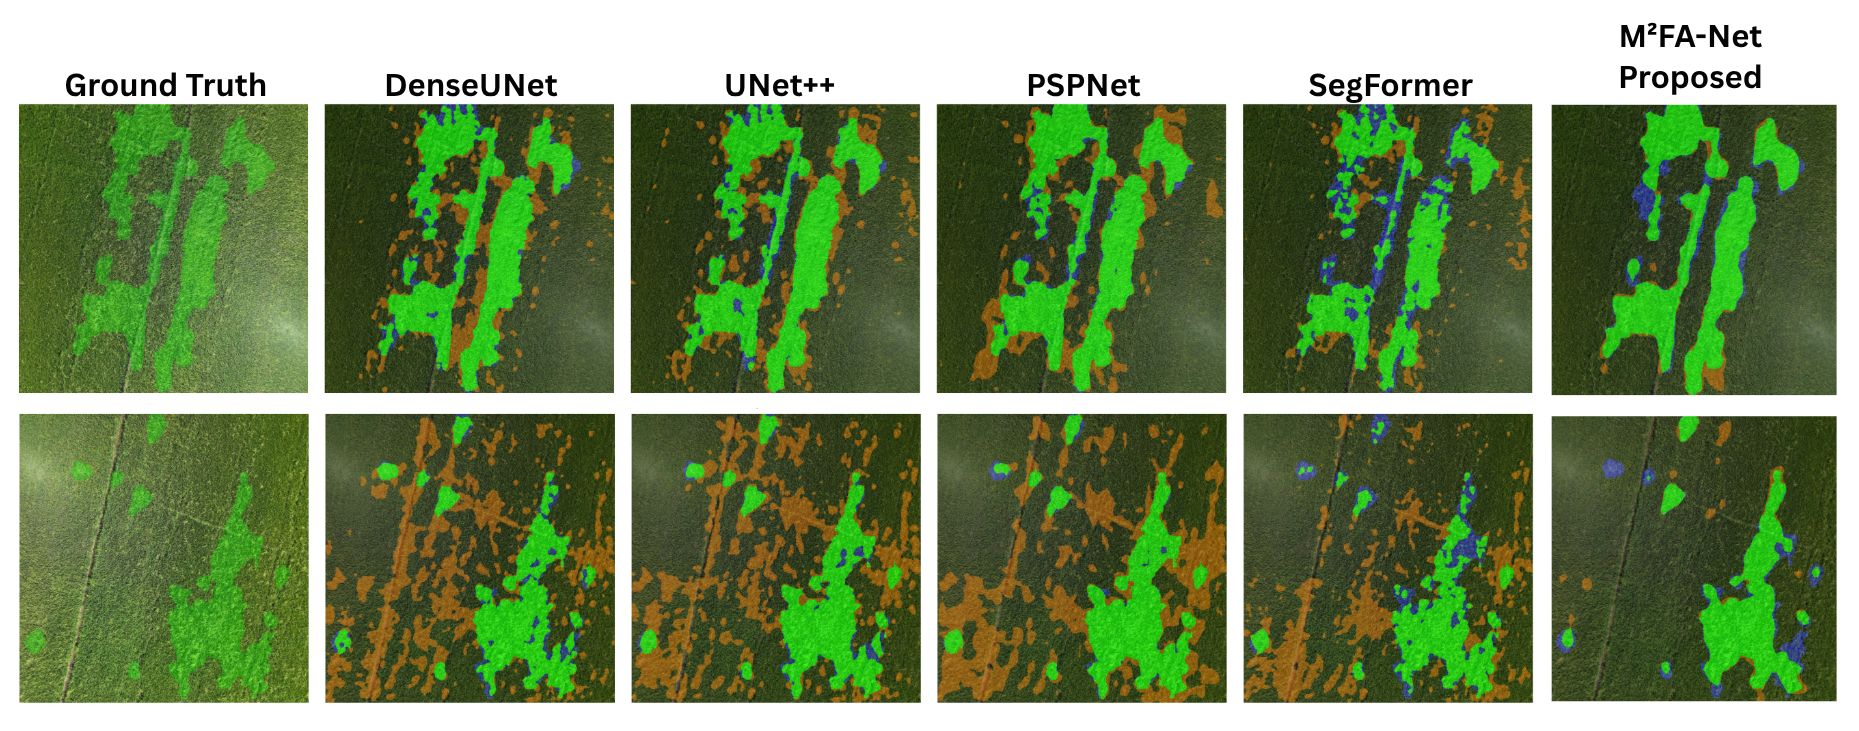
\includegraphics[width=\linewidth]{Images/Comparison_new.png}
\caption{Qualitative comparison of crop-weed segmentation results produced by different state-of-the-art models on representative field samples. The proposed $M^2$FA-Net generates cleaner segmentation masks with improved structural consistency, sharper boundary localization, and significantly fewer segmentation artifacts compared to DenseUNet, U-Net++, PSPNet, and SegFormer, particularly in dense vegetation and sparse weed regions.}
\label{fig:comparison}
\end{figure*}

\begin{table*}[t]

\setlength{\tabcolsep}{4pt}
\caption{Performance comparison of different models for crop-weed segmentation. Results are reported as mean $\pm$ standard deviation (in \%).}
\label{tab:results}
\resizebox{\textwidth}{!}{%
\begin{tabular}{lccccc}
\hline
\textbf{Method} & \textbf{Accuracy (\%)} & \textbf{Precision (\%)} & \textbf{Recall (\%)} & \textbf{IoU (\%)} & \textbf{Dice (\%)} \\
\hline

U-Net \cite{ronneberger2015unet}
& 89.68 $\pm$ 0.40 
& 82.18 $\pm$ 2.59 
& 80.44 $\pm$ 2.36 
& 68.75 $\pm$ 0.46 
& 80.97 $\pm$ 0.33 \\

Transformer (ViT) \cite{dosovitskiy2021vit}
& 82.48 $\pm$ 0.57 
& 66.99 $\pm$ 1.94 
& 76.78 $\pm$ 2.45 
& 56.08 $\pm$ 0.20
& 70.87 $\pm$ 0.19 \\

HRNet \cite{sun2019high}
& 81.67 $\pm$ 0.62 
& 63.48 $\pm$ 1.88 
& 73.21 $\pm$ 2.76 
& 52.72 $\pm$ 0.41 
& 67.36 $\pm$ 0.43 \\

PSPNet \cite{zhao2017pyramid}
& 89.87 $\pm$ 0.33 
& 79.82 $\pm$ 1.35 
& 83.27 $\pm$ 1.61 
& 69.34 $\pm$ 0.59 
& 81.36 $\pm$ 0.40 \\



DeepLabV3 \cite{chen2018Deeplabv3plus}
& 88.89 $\pm$ 0.24 
& 79.81 $\pm$ 2.11 
& 80.23 $\pm$ 2.43 
& 66.95 $\pm$ 0.54 
& 79.62 $\pm$ 0.41 \\


CRF-U-Net \cite{sahin2023segmentation}
& 88.91 $\pm$ 0.89 
& 80.11 $\pm$ 2.01 
& 79.76 $\pm$ 3.86 
& 66.82 $\pm$ 2.55 
& 79.54 $\pm$ 1.93 \\

SegFormer \cite{xie2021segformer}
& 86.04 $\pm$ 0.63 
& 78.65 $\pm$ 2.23 
& 70.58 $\pm$ 3.54 
& 59.04 $\pm$ 1.87 
& 73.13 $\pm$ 1.56 \\

CNN + Transformer \cite{guo2025cnn_transformer}
& 88.36 $\pm$ 0.52 
& 74.39 $\pm$ 1.81 
& 80.59 $\pm$ 1.53 
& 63.55 $\pm$ 0.65 
& 76.30 $\pm$ 0.55 \\

Swin Transformer \cite{liu2021swin}
& 90.58 $\pm$ 0.39 
& 85.99 $\pm$ 2.19 
& 86.13 $\pm$ 2.83 
& 75.43 $\pm$ 1.03 
& 85.99 $\pm$ 0.67 \\

U-Net++ \cite{zhou2018unet++}
& 90.41 $\pm$ 0.13 
& 80.28 $\pm$ 2.16 
& 78.26 $\pm$ 1.81 
& 66.39 $\pm$ 0.27 
& 78.56 $\pm$ 0.22 \\

DenseUNet \cite{mu2023densenet}
& 90.75 $\pm$ 0.26
& 83.77 $\pm$ 2.88 
& 81.38 $\pm$ 2.78 
& 70.67 $\pm$ 0.31 
& 82.27 $\pm$ 0.23 \\

\textbf{$M^2$FA-Net(Proposed)}
& \textbf{94.06 $\pm$ 0.07} 
& \textbf{90.72 $\pm$ 0.69}
& \textbf{87.82 $\pm$ 0.84} 
& \textbf{80.79 $\pm$ 0.24} 
& \textbf{89.21 $\pm$ 0.15} \\

\hline
\end{tabular}
}
\end{table*}



DeepLab-based architectures further improve segmentation performance through multi-scale contextual aggregation using dilated convolutions. DeepLabV3 achieves 66.95\% IoU and 79.62\% Dice, outperforming several CNN and transformer-based approaches. This demonstrates the effectiveness of multi-scale feature extraction and contextual learning for agricultural segmentation tasks. However, convolution-only approaches still face challenges in modeling complex multimodal feature interactions. 
In contrast, the proposed $M^2$FA-Net achieves the best performance across all evaluation metrics, obtaining 94.06\% accuracy, 90.72\% precision, 87.82\% recall, 80.79\% IoU, and 89.21\% Dice score. Compared with Swin Transformer, the
strongest competing baseline, the proposed
$M^2$FA-Net improves IoU by 5.36 percentage
points and Dice score by 3.22 percentage
points. The proposed framework also outperforms DeepLabV3 by 13.84\% in IoU and 9.59\% in Dice score. In addition, $M^2$FA-Net has the highest recall among all methods, indicating the reduction of false negatives and improvement of the weed detection capability, which is important for precision agriculture applications.

\begin{table*}[t]
    \centering
    
    \small
    \setlength{\tabcolsep}{4pt}
    \renewcommand{\arraystretch}{1.2}
    \caption{Statistical comparison of $M^2$FA-Net against selected baselines using two-sided Welch's $t$-tests on five independent runs. Improvements and confidence intervals are in percentage points. $p_{\mathrm{Holm}}$ is adjusted across 10 comparisons (five baselines $\times$ two metrics). The 95\% confidence intervals are unadjusted individual intervals.}
    \label{tab:stat_significance}
    \resizebox{\textwidth}{!}{%
    \begin{tabular}{lccc ccc}
    \hline
   \textbf{Baseline}
& \multicolumn{3}{c}{IoU}
& \multicolumn{3}{c}{Dice} \\

\hline
    & \textbf{Gain (pp)} & \textbf{95\% CI (pp)} & \textbf{$p_{\mathrm{Holm}}$} & \textbf{Gain (pp)} & \textbf{95\% CI (pp)} & \textbf{$p_{\mathrm{Holm}}$} \\
    \hline
    U-Net & 12.04 & [11.47, 12.61] & $2.56\times 10^{-8}$ & 8.24 & [7.84, 8.64] & $8.11\times 10^{-8}$ \\
    SegFormer & 21.75 & [19.44, 24.06] & $4.04\times 10^{-5}$ & 16.08 & [14.15, 18.01] & $5.51\times 10^{-5}$ \\
    DeepLabV3 & 13.84 & [13.18, 14.50] & $8.11\times 10^{-8}$ & 9.59 & [9.09, 10.09] & $2.88\times 10^{-7}$ \\
    U-Net++ & 14.40 & [14.03, 14.77] & $3.88\times 10^{-12}$ & 10.65 & [10.37, 10.93] & $4.33\times 10^{-11}$ \\
    Swin Transformer & 5.36 & [4.10, 6.62] & $3.87\times 10^{-4}$ & 3.22 & [2.40, 4.04] & $3.87\times 10^{-4}$ \\
    \hline
    \end{tabular}}
\end{table*}


To examine the reliability of the observed performance gains, we compared $M^2$FA-Net with U-Net, SegFormer, DeepLabV3, U-Net++, and Swin Transformer using two-sided Welch's $t$-tests on the mean and sample standard deviation from five independent runs per model. Holm correction was applied across all ten IoU and Dice comparisons. As shown in Table~\ref{tab:stat_significance}, the proposed method achieved statistically significant improvements over all five baselines for both metrics (all Holm-adjusted $p<0.001$). Against the strongest IoU baseline, Swin Transformer, the improvement was 5.36 percentage points in IoU (95\% CI: [4.10, 6.62]) and 3.22 points in Dice (95\% CI: [2.40, 4.04]). These findings provide statistical evidence
that the observed performance improvements are
consistent across repeated training runs on the
evaluated test split. However, they do not
establish generalization to spatially independent
fields or acquisition conditions.


As shown in the first sample in Fig.~\ref{fig:comparison}, most baseline methods fail to distinguish weeds from cultivated rice due to the strong visual similarity in terms of texture and color. PSPNet shows aggressive over-segmentation, and SegFormer produces sparse false activations in dense vegetation regions. The proposed $M^2$FA-Net, on the other hand, produces smoother and more coherent segmentation masks, with sharper boundaries and substantially fewer misclassification errors. The second sample shows a more difficult situation with scarce and dispersed weed regions. Existing approaches are not able to model thin weed structures accurately and tend to classify surrounding background areas as weeds, leading to noisy predictions and more false negatives. In contrast, the proposed $M^2$FA-Net can accurately detect both large and small weed regions with good boundary preservation and low background noise. 

\begin{figure*}[p]
    \centering
    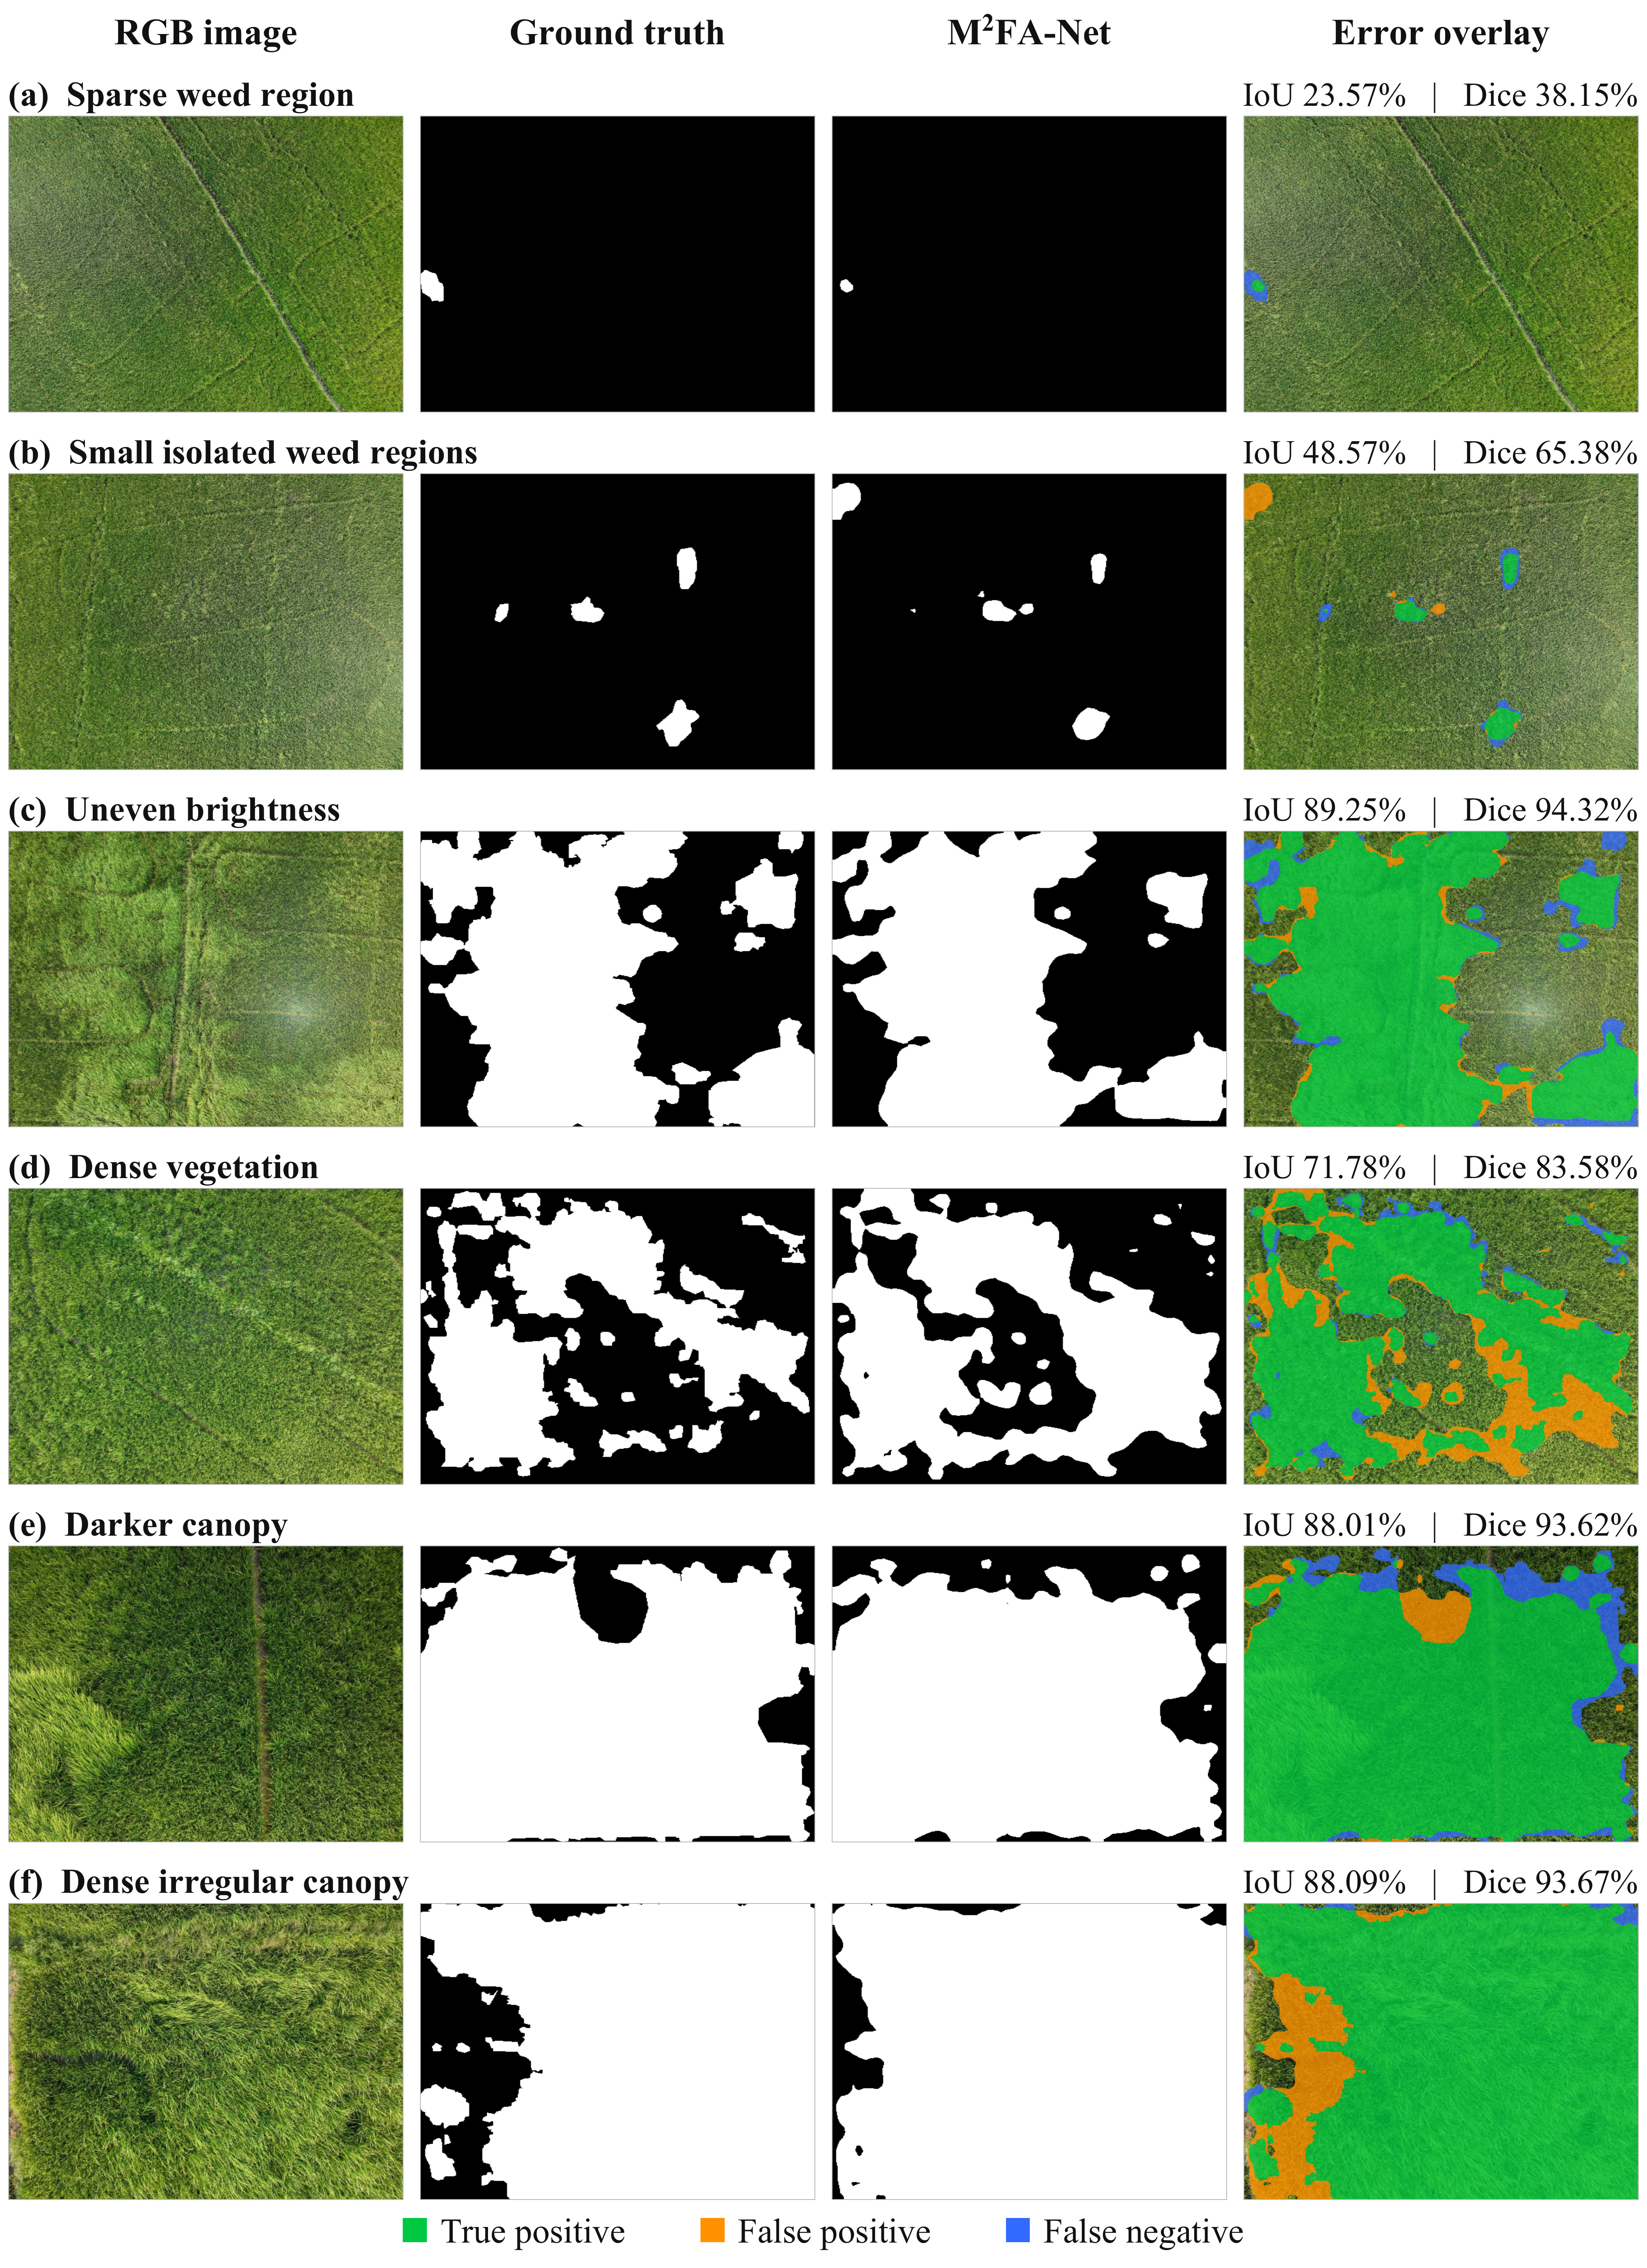
\includegraphics[
        width=\textwidth,
        height=0.85\textheight,
        keepaspectratio
    ]{Images/figure_qualitative_six_cases.png}
    \caption{Qualitative evaluation of
    $M^2$FA-Net under challenging field conditions.
    The examples include sparse weed regions,
    small isolated weeds, uneven illumination,
    and dense vegetation. The error overlays
    distinguish true positives (green),
    false positives (orange), and false
    negatives (blue). Per-image IoU and Dice
    scores are also reported.}
    \label{fig:challenging_cases}
\end{figure*}


To further examine the proposed
framework, Fig.~\ref{fig:challenging_cases}
presents additional qualitative examples under
challenging field conditions. The model exhibits
considerable difficulty in detecting sparse and
small isolated weed regions, achieving IoU scores
of 23.57\% and 48.57\%, respectively. These cases
reveal missed weed regions and occasional false
detections. Dense vegetation also introduces
segmentation errors, particularly around
irregular boundaries. However, the model maintains
relatively accurate predictions in several
examples involving uneven illumination and
complex canopy structures. These observations
highlight both the segmentation capabilities
and the limitations of $M^2$FA-Net under
different field conditions.


\subsection{Ablation Study of
\texorpdfstring{$M^2$FA-Net}{M2FA-Net}}
To evaluate the effectiveness of each component in the proposed $M^2$FA-Net framework, an ablation study is conducted by systematically removing individual modules, including multi-level fusion, CBAM attention, deep supervision, warmup scheduling, and data augmentation, and is given in Table~\ref{tab:ablation}. The Baseline (Early Fusion) combines RGB and multispectral inputs before feature extraction using a shared encoder, whereas the No Multi-Level Fusion configuration retains separate modality-specific encoders and combines their features only at the final encoder stage. In contrast, the proposed $M^2$FA-Net performs hierarchical feature fusion at all four encoder stages. For improved interpretability, the corresponding IoU and Dice
trends are additionally visualized in Fig.~\ref{fig:iou}, while
Fig.~\ref{fig:component_contribution} summarizes the relative
contribution of each architectural component.
As shown in Fig.~\ref{fig:iou}, the complete
$M^2$FA-Net achieves the highest IoU and Dice scores,
while removing individual components reduces
segmentation performance. The largest reduction
occurs when multi-level fusion is removed,
highlighting the importance of hierarchical
spatial-spectral feature integration.
Fig.~\ref{fig:component_contribution} further
illustrates the contributions of the remaining
components, particularly deep supervision
and CBAM attention.
\begin{table*}[t]
\centering

\caption{Ablation study of the architectural
and training components of $M^2$FA-Net.
Results are reported as mean $\pm$
standard deviation (in \%).}

\label{tab:ablation}
\resizebox{\textwidth}{!}{%

\begin{tabular}{lccccc}
\hline
\textbf{Method} & \textbf{Accuracy (\%)} & \textbf{Precision (\%)} & \textbf{Recall (\%)} & \textbf{IoU (\%)} & \textbf{Dice (\%)} \\
\hline

Baseline (Early Fusion) 
& 92.75 $\pm$ 0.09
& 90.28 $\pm$ 0.42
& 82.98 $\pm$ 0.43 
& 76.48 $\pm$ 0.25 
& 86.41 $\pm$ 0.15 \\

No Multi-Level Fusion
& 92.86 $\pm$ 0.09 
& 90.81 $\pm$ 0.56 
& 82.80 $\pm$ 0.92 
& 76.68 $\pm$ 0.42 
& 86.55 $\pm$ 0.28 \\

No CBAM Attention 
& 93.10 $\pm$ 0.11
& 90.61 $\pm$ 0.80 
& 84.10 $\pm$ 0.98
& 77.62 $\pm$ 0.38
& 87.18 $\pm$ 0.25 \\

No Deep Supervision  
& 93.06 $\pm$ 0.14 
& 90.95 $\pm$ 0.67 
& 83.36 $\pm$ 0.99
& 77.24 $\pm$ 0.51 
& 86.92 $\pm$ 0.34 \\

No Warmup Scheduler
& 92.78 $\pm$ 0.40
& 90.92 $\pm$ 1.80
& 83.10 $\pm$ 3.08
& 76.90 $\pm$ 1.38 
& 86.72 $\pm$ 0.91 \\

No Augmentation   
& 93.26 $\pm$ 0.08 
& 90.60 $\pm$ 0.28
& 84.78 $\pm$ 0.43 
& 78.18 $\pm$ 0.24
& 87.55 $\pm$ 0.15 \\

\textbf{\boldmath$M^2$FA-Net (proposed)}
& \textbf{94.06 $\pm$ 0.07} 
& \textbf{90.72 $\pm$ 0.69} 
& \textbf{87.82 $\pm$ 0.84} 
& \textbf{80.79 $\pm$ 0.24} 
& \textbf{89.21 $\pm$ 0.15} \\

\hline
\end{tabular}
}
\end{table*}
\begin{figure}[t]
    \centering
    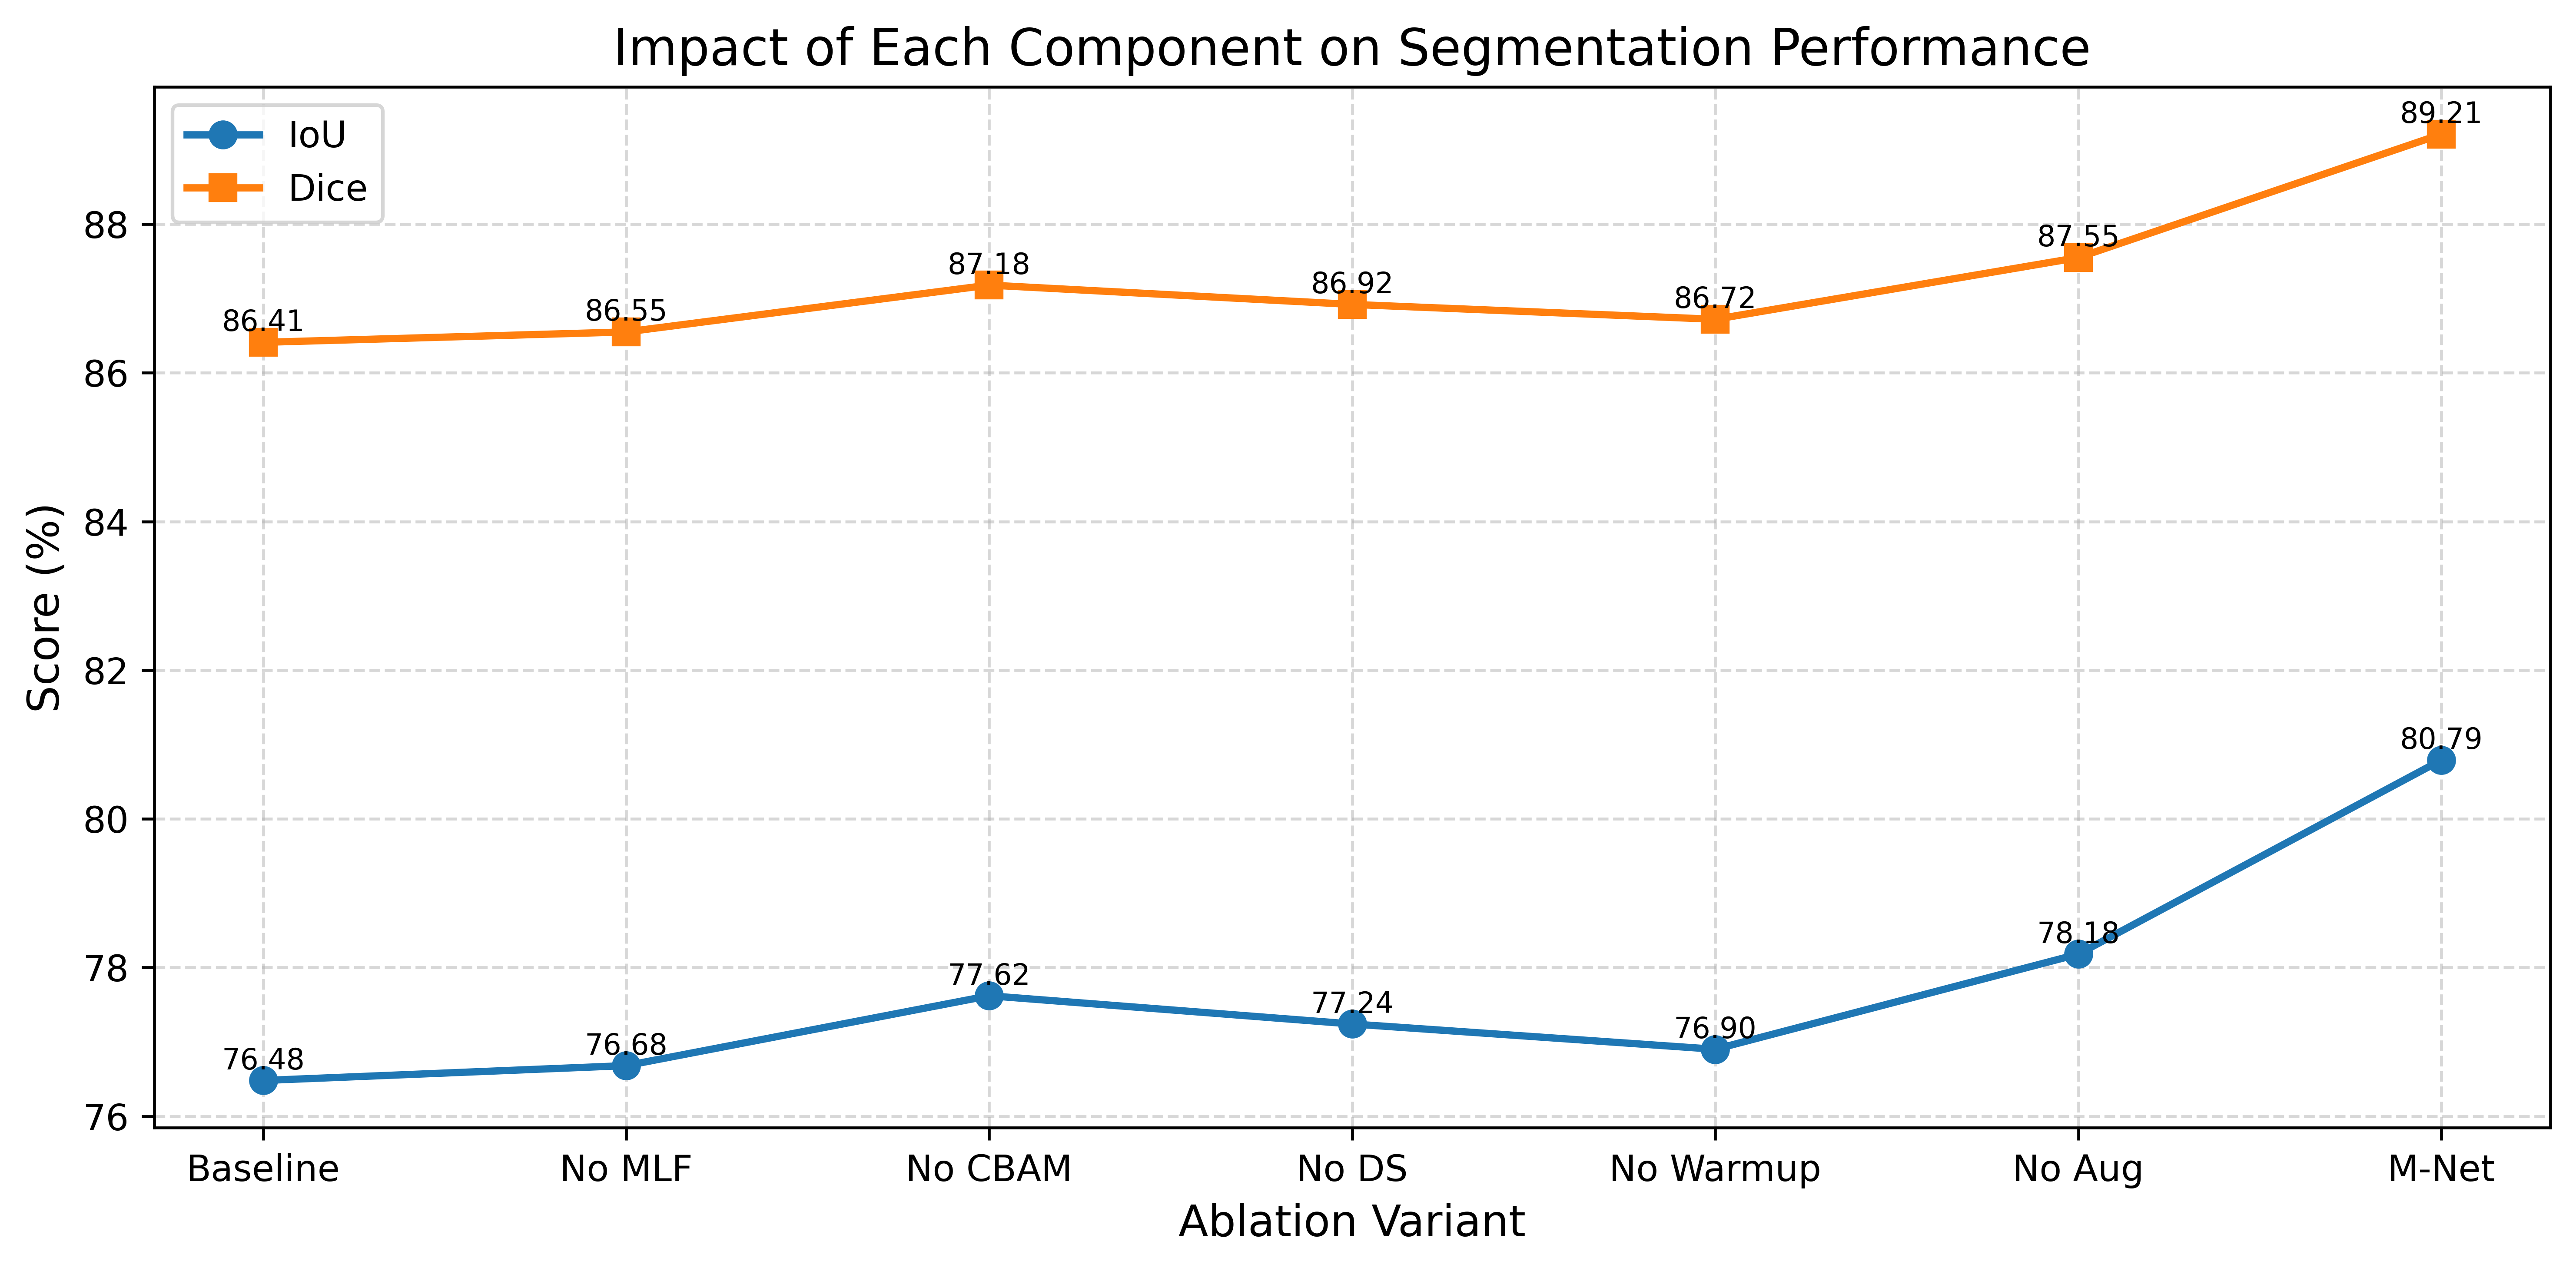
\includegraphics[width=12cm]{Images/ablation_iou_dice (2).png}
\caption{Comparison of IoU and Dice scores
across different ablation configurations
of $M^2$FA-Net.}
    \label{fig:iou}
\end{figure}
\begin{figure}[t]
    \centering
    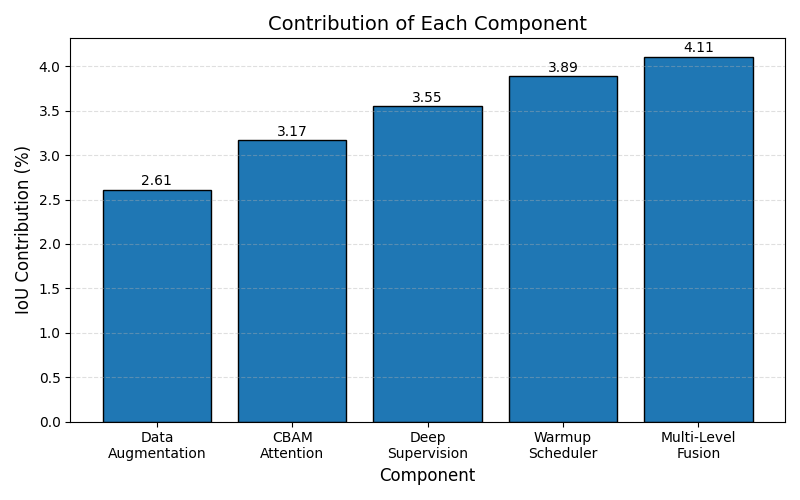
\includegraphics[width=12cm]{Images/contribution.png}
\caption{Relative contribution of individual
components to the IoU performance of $M^2$FA-Net.}
    \label{fig:component_contribution}
\end{figure}






\subsection{Input-Modality Ablation}
\label{sec:modality}

To quantify the contribution of different input
modalities, four configurations are evaluated:
(i) RGB only; (ii) RGB with four multispectral
bands (MS4: G, R, RE, NIR); (iii) RGB with MS4
and NDVI; and (iv) RGB with MS4, NDVI, and NDRE
(the full-input configuration). The RGB-only
configuration employs a single RGB encoder,
whereas the remaining configurations retain
the dual-stream architecture with multi-level
feature fusion and the corresponding
multispectral input channels. Within this
ablation study, the loss function, training
schedule, data augmentation, and auxiliary
supervision are kept consistent across the
configurations. Results are reported as mean
$\pm$ standard deviation over five runs with
different random seeds.
Fig.~\ref{fig:modality} presents the results.


Adding the four multispectral bands raises IoU from 83.11\% to 83.75\% (+0.64 points) and Dice from 90.77\% to 91.15\% (+0.38 points). The gain is small in absolute terms, but it comes with a marked reduction in run-to-run variability: the IoU standard deviation drops from 1.24 to 0.10. Adding NDVI changes IoU by $-0.07$ points, and adding NDRE on top of NDVI changes it by $+0.13$ points; both changes are smaller than the standard deviation of the corresponding runs. The vegetation indices therefore give no measurable improvement beyond the raw bands in our setting, which is plausible because both indices are deterministic functions of bands that the network already receives. Since the RGB-only runs vary more than the gap to the multispectral settings, we regard the improvement from the bands as consistent in direction but modest, and we do not claim a statistically significant difference.



The input-modality ablation was conducted as a
separate experimental analysis using the same
dataset partitions, loss function, and training
duration as the main experiments. However, minor
implementation differences existed in the
initialization of the multispectral encoder and
checkpoint selection. Specifically, the
input-modality experiments evaluated the best
validation-selected checkpoints, whereas the
main experiments evaluated the final-epoch
models. Consequently, the absolute performance
values of the full-input configuration differ
between the two experiments. The contribution
of each input modality is therefore assessed
through comparisons within the consistent
input-modality ablation protocol.



\begin{figure}[t]
\centering
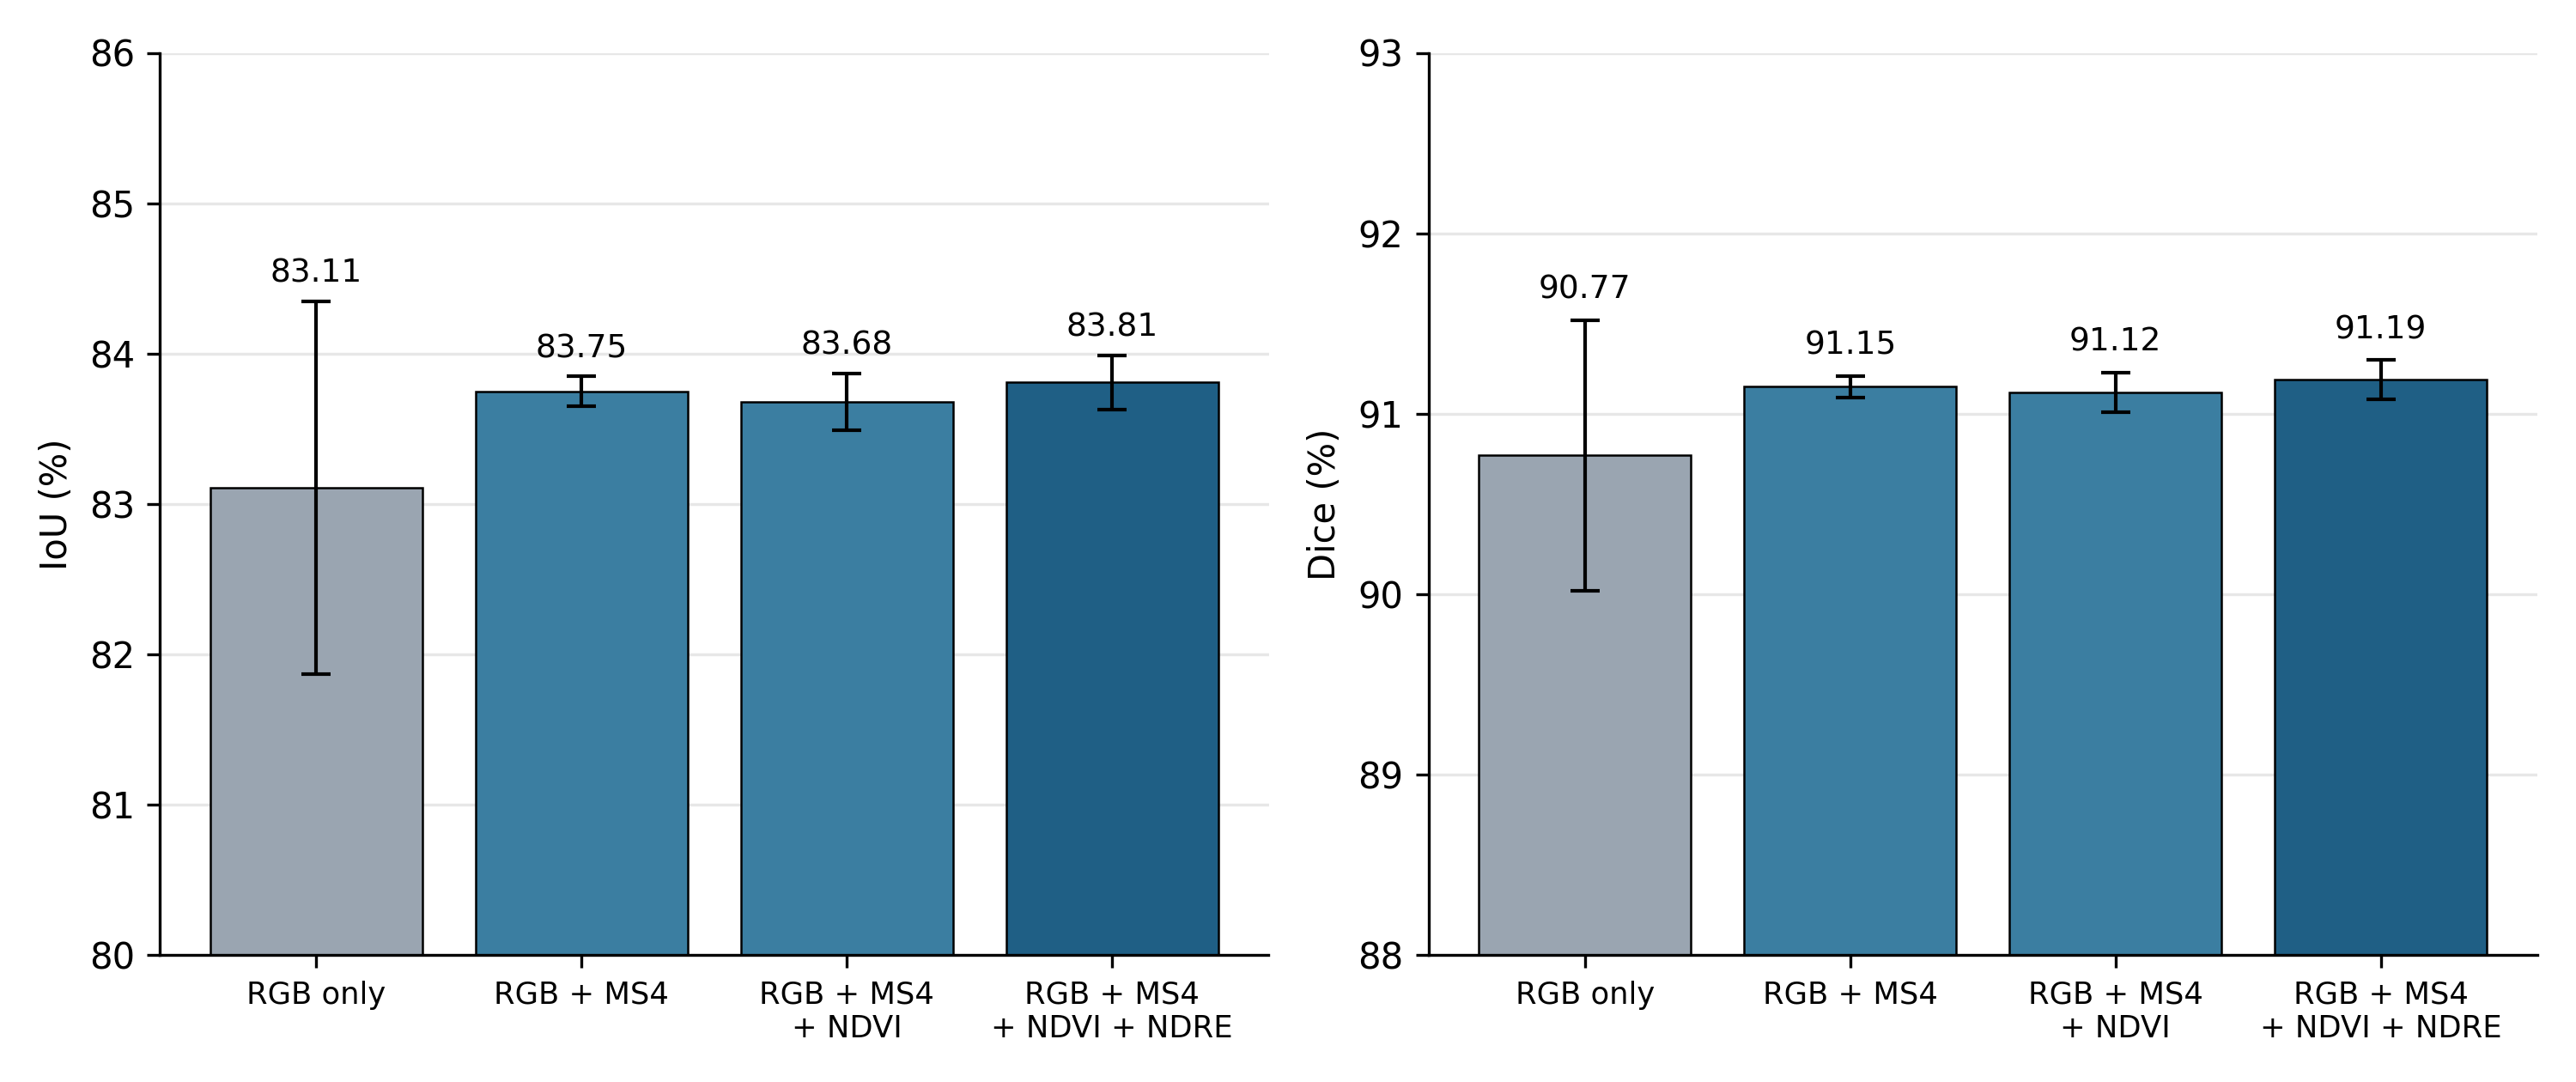
\includegraphics[width=\linewidth]{Images/modality_ablation.png}
\caption{Input-modality ablation: IoU (left) and Dice (right) for the four input settings. Bars show the mean and error bars the standard deviation over repeated runs; the vertical axes are truncated to make small differences visible.}
\label{fig:modality}
\end{figure}



\subsection{Computational Complexity Analysis}

To further evaluate the efficiency of the proposed framework, a computational complexity analysis was conducted in terms of the number of parameters, floating point operations (FLOPs), and inference speed measured in frames per second (FPS). All complexity metrics were computed using an input resolution of $512 \times 512$, while FPS was measured using batch size 1 under inference mode using the same hardware configuration described in Section IV.


\begin{table}[htbp]
\centering
\caption{Computational complexity comparison of different segmentation models in terms of FLOPs and inference speed}
\label{tab:complexity}
\begin{tabular}{lcc}
\hline
Model & FLOPs (G) & Inference Speed(FPS)\\
\hline
DenseUNet  & 68.60 & 47.00 \\
U-Net++  & 148.29 & 40.81 \\
PSPNet  & 19.53 & 280.11 \\
SegFormer  & 6.77 & 194.58 \\
$M^2$FA-Net (Proposed)  & 267.68 & 40.22 \\
\hline
\end{tabular}
\end{table}

\begin{figure}[t]
    \centering
    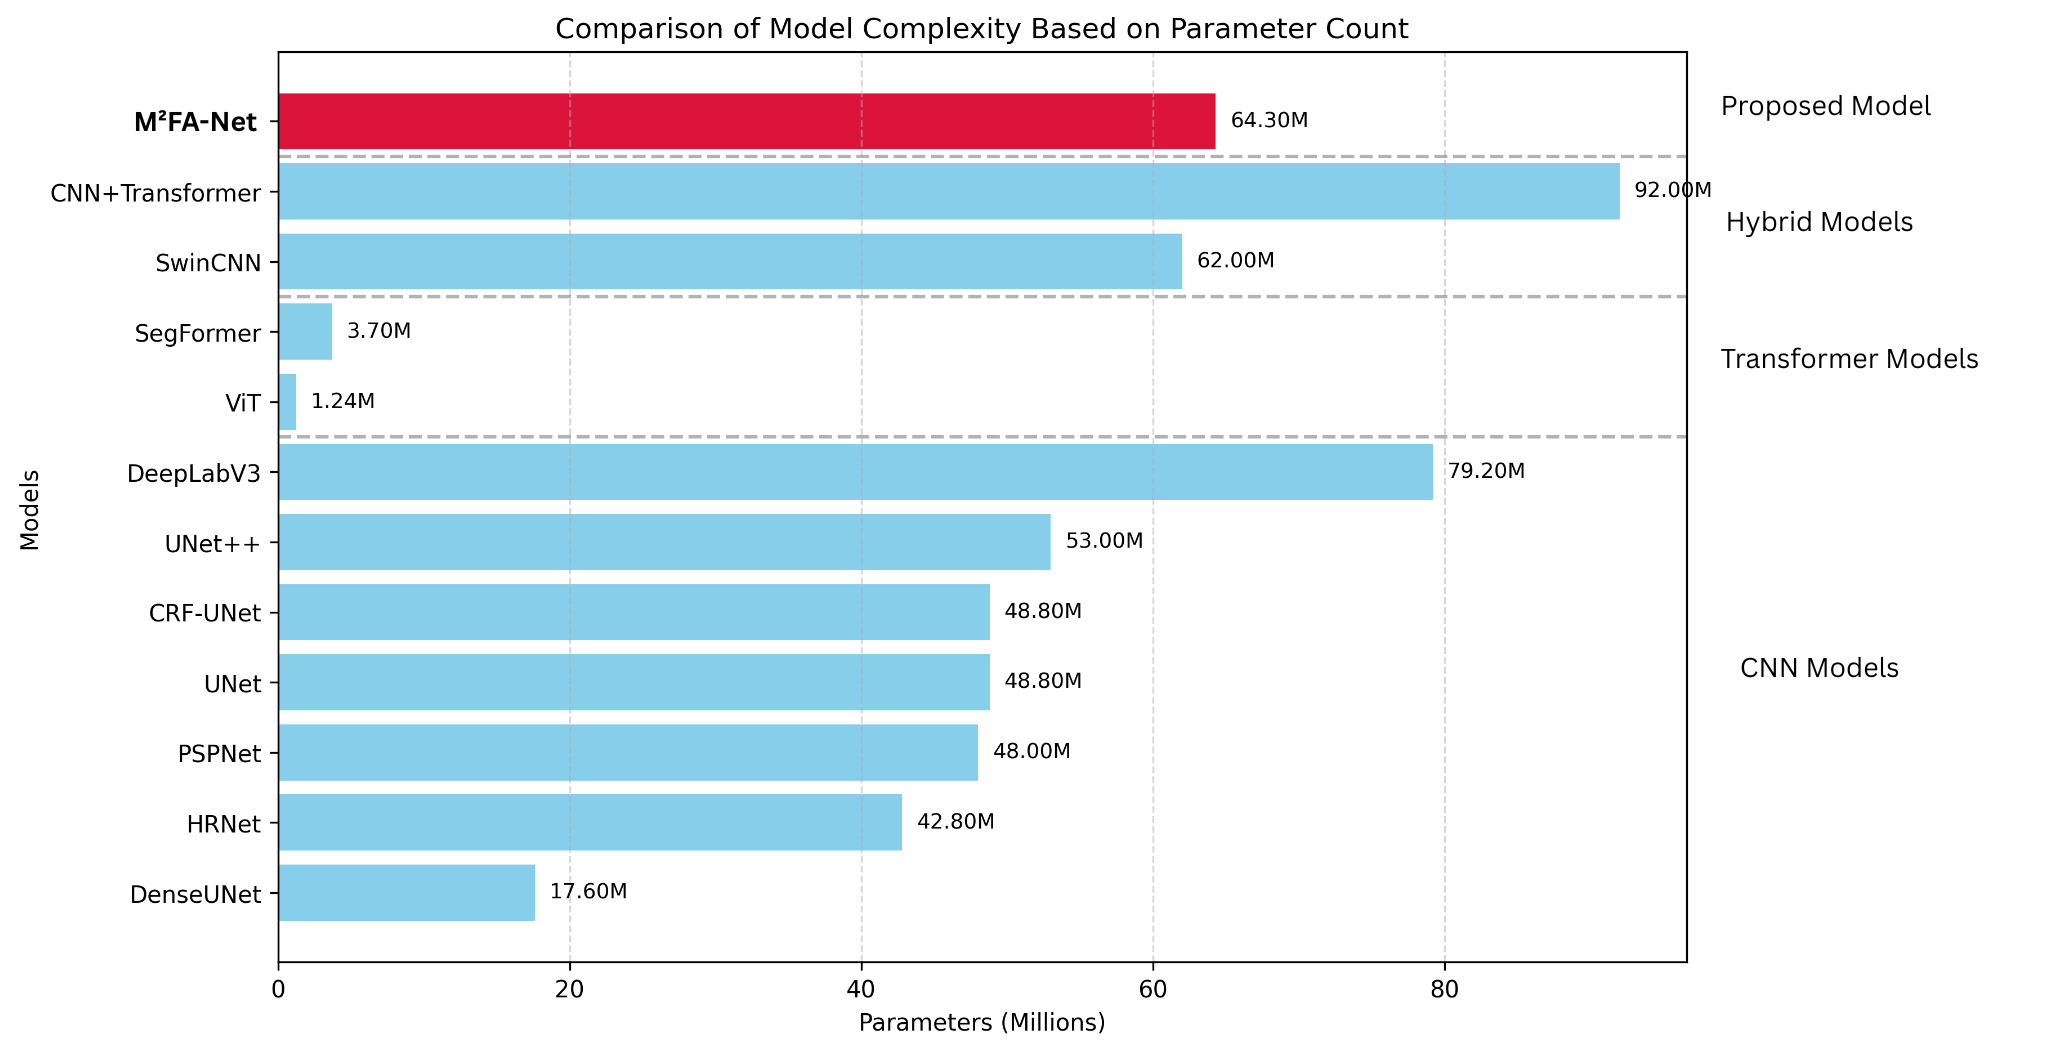
\includegraphics[width=17cm]{Images/parameters.png}
    % Parameter Comparison
\caption{Comparison of model complexity in terms of parameter count across representative CNN-based, transformer-based, hybrid, and proposed architectures. Although $M^2$FA-Net contains more parameters than several baseline models, it remains substantially lighter than some transformer-hybrid frameworks while achieving superior segmentation performance.}
    \label{fig:parameter}
\end{figure}

Table~\ref{tab:complexity} presents the computational complexity comparison of different segmentation models in terms of FLOPs and inference speed. Figure~\ref{fig:parameter} further compares the parameter count of representative segmentation architectures. Although the proposed framework is computationally more demanding than lightweight architectures such as PSPNet and SegFormer, it still maintains competitive inference speed while delivering significantly superior segmentation accuracy. Taking into account substantial improvements in IoU and Dice score, the additional computational cost is justified for precision agriculture applications where segmentation quality is of primary importance. Overall, the proposed $M^2$FA-Net achieves improved segmentation performance at the cost of increased computational complexity. Therefore, further optimization and hardware-specific evaluation are necessary before considering deployment on resource-constrained UAV platforms.

The reported inference speed of 40.22 FPS was obtained on a desktop NVIDIA RTX A5000 GPU and should not be interpreted as evidence of real-time inference capability on UAV or edge devices. Future work will investigate device-specific inference latency, GPU memory consumption, and deployment feasibility on platforms such as NVIDIA Jetson.




\subsection{Hyperparameter Sensitivity Analysis}
To further investigate the robustness of the proposed $M^2$FA-Net framework, a series of hyperparameter sensitivity experiments is conducted. Key training parameters, including learning rate, batch size, auxiliary loss weight, warmup epochs, weight decay, and loss function weights, were systematically varied while keeping all other settings unchanged. 
Fig.~\ref{fig:batch_analysis} reveals the effects of batch sizes on segmentation results. The highest performance among the evaluated settings is achieved with a batch size of 8, which was adopted for all subsequent experiments.
Figure~\ref{fig:aux_analysis} shows that increasing the auxiliary loss weight consistently improves segmentation performance. The best performance is achieved at $\lambda=0.7$, which was adopted in the final $M^2$FA-Net framework.
As illustrated in Fig.~\ref{fig:learning_rate}, the results improve significantly when increasing the learning rate from $1\times10^{-5}$, reaching its highest performance at $2\times10^{-4}$, which was selected for the final configuration of the model.



 According to the obtained data, weight decay, warmup epochs, and loss weights have only a slight effect on segmentation efficiency in comparison with the learning rate, batch size, and auxiliary loss weight. For the weight decay parameter within its range from $10^{-5}$ to 1, the difference in val IoU did not exceed 0.5\%. Likewise, variations in the number of warmup epochs between 0 and 5 had only a negligible effect on the framework's performance; the warmup stage of 3 epochs was finally used. Besides, several different loss function weightings for CE, Dice, and Boundary losses led to almost similar results and proved the framework's insensitivity to the specified parameter. Among them, the combination with weights of 0.4 for CE, 0.4 for Dice, and 0.2 for Boundary was recognized as the best one.

\begin{figure*}[t]
\centering
% Top row
\begin{subfigure}[t]{0.48\textwidth}
    \centering
    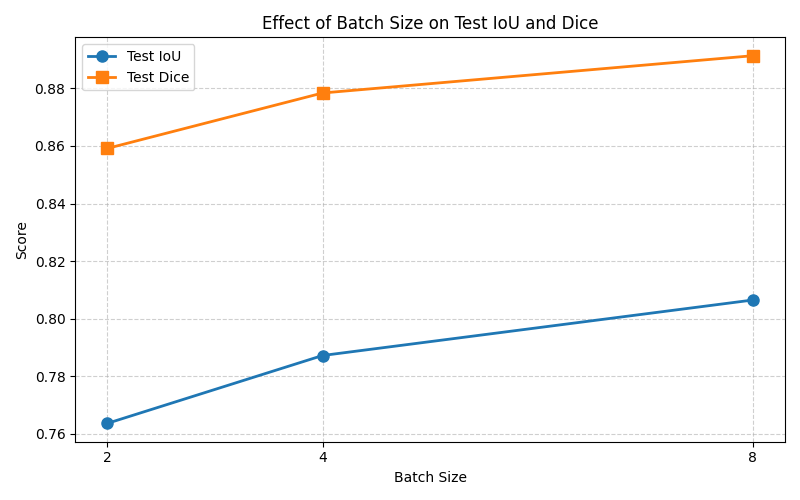
\includegraphics[width=\linewidth]{Images/batchsize_ioudice.png}
\caption{Batch size sensitivity.}
    \label{fig:batch_analysis}
\end{subfigure}
\hfill
\begin{subfigure}[t]{0.48\textwidth}
    \centering
    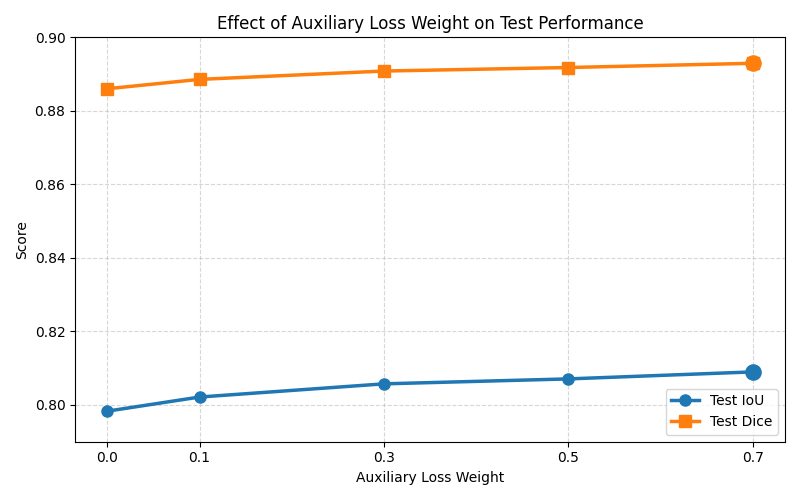
\includegraphics[width=\linewidth]{Images/auxclassifer.png}
\caption{Auxiliary loss weight sensitivity.}
    \label{fig:aux_analysis}
\end{subfigure}

\vspace{0.5cm}

% Bottom row centered
\begin{subfigure}{0.6\textwidth}
    \centering
    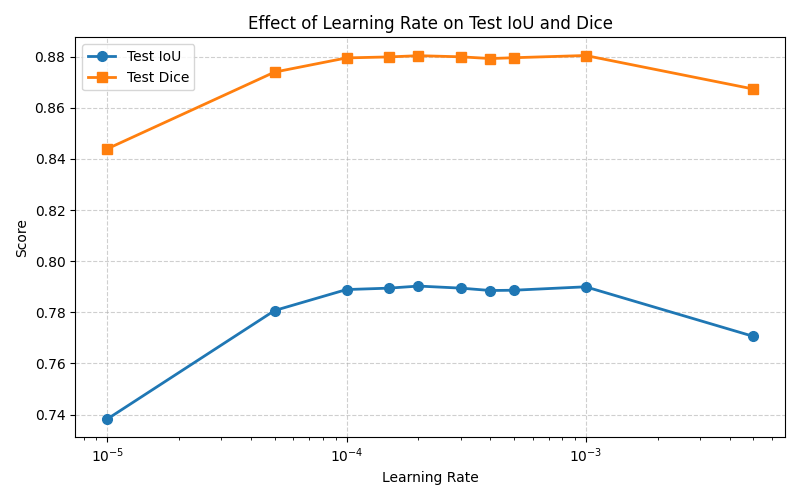
\includegraphics[width=\linewidth]{Images/learningrate_iouudice.png}
\caption{Learning rate sensitivity.}
    \label{fig:learning_rate}
\end{subfigure}

\caption{Hyperparameter sensitivity analysis of the proposed $M^2$FA-Net.}
\label{fig:hyperparameter_analysis}

\end{figure*}

To analyze the optimization behavior of the proposed framework,
the evolution of training and validation losses is monitored
throughout the training process. As shown in Fig.~\ref{fig:loss_curves},
both losses decrease steadily across epochs, indicating stable
convergence and effective optimization. Furthermore, the small
gap between the training and validation curves suggests 
a relatively small difference between
training and validation losses under the
evaluated data partition. However, these
curves alone do not establish generalization
to spatially independent field observations.
In addition to loss convergence, segmentation performance is
tracked using validation IoU and Dice metrics. As illustrated in
Fig.~\ref{fig:iou_dice}, both metrics improve consistently
throughout training before stabilizing during the later epochs.
The steady increase in validation performance confirms the
effectiveness of the proposed training strategy and optimization
settings.

\begin{figure*}[t]
\centering

\begin{subfigure}[t]{0.48\textwidth}
    \centering
    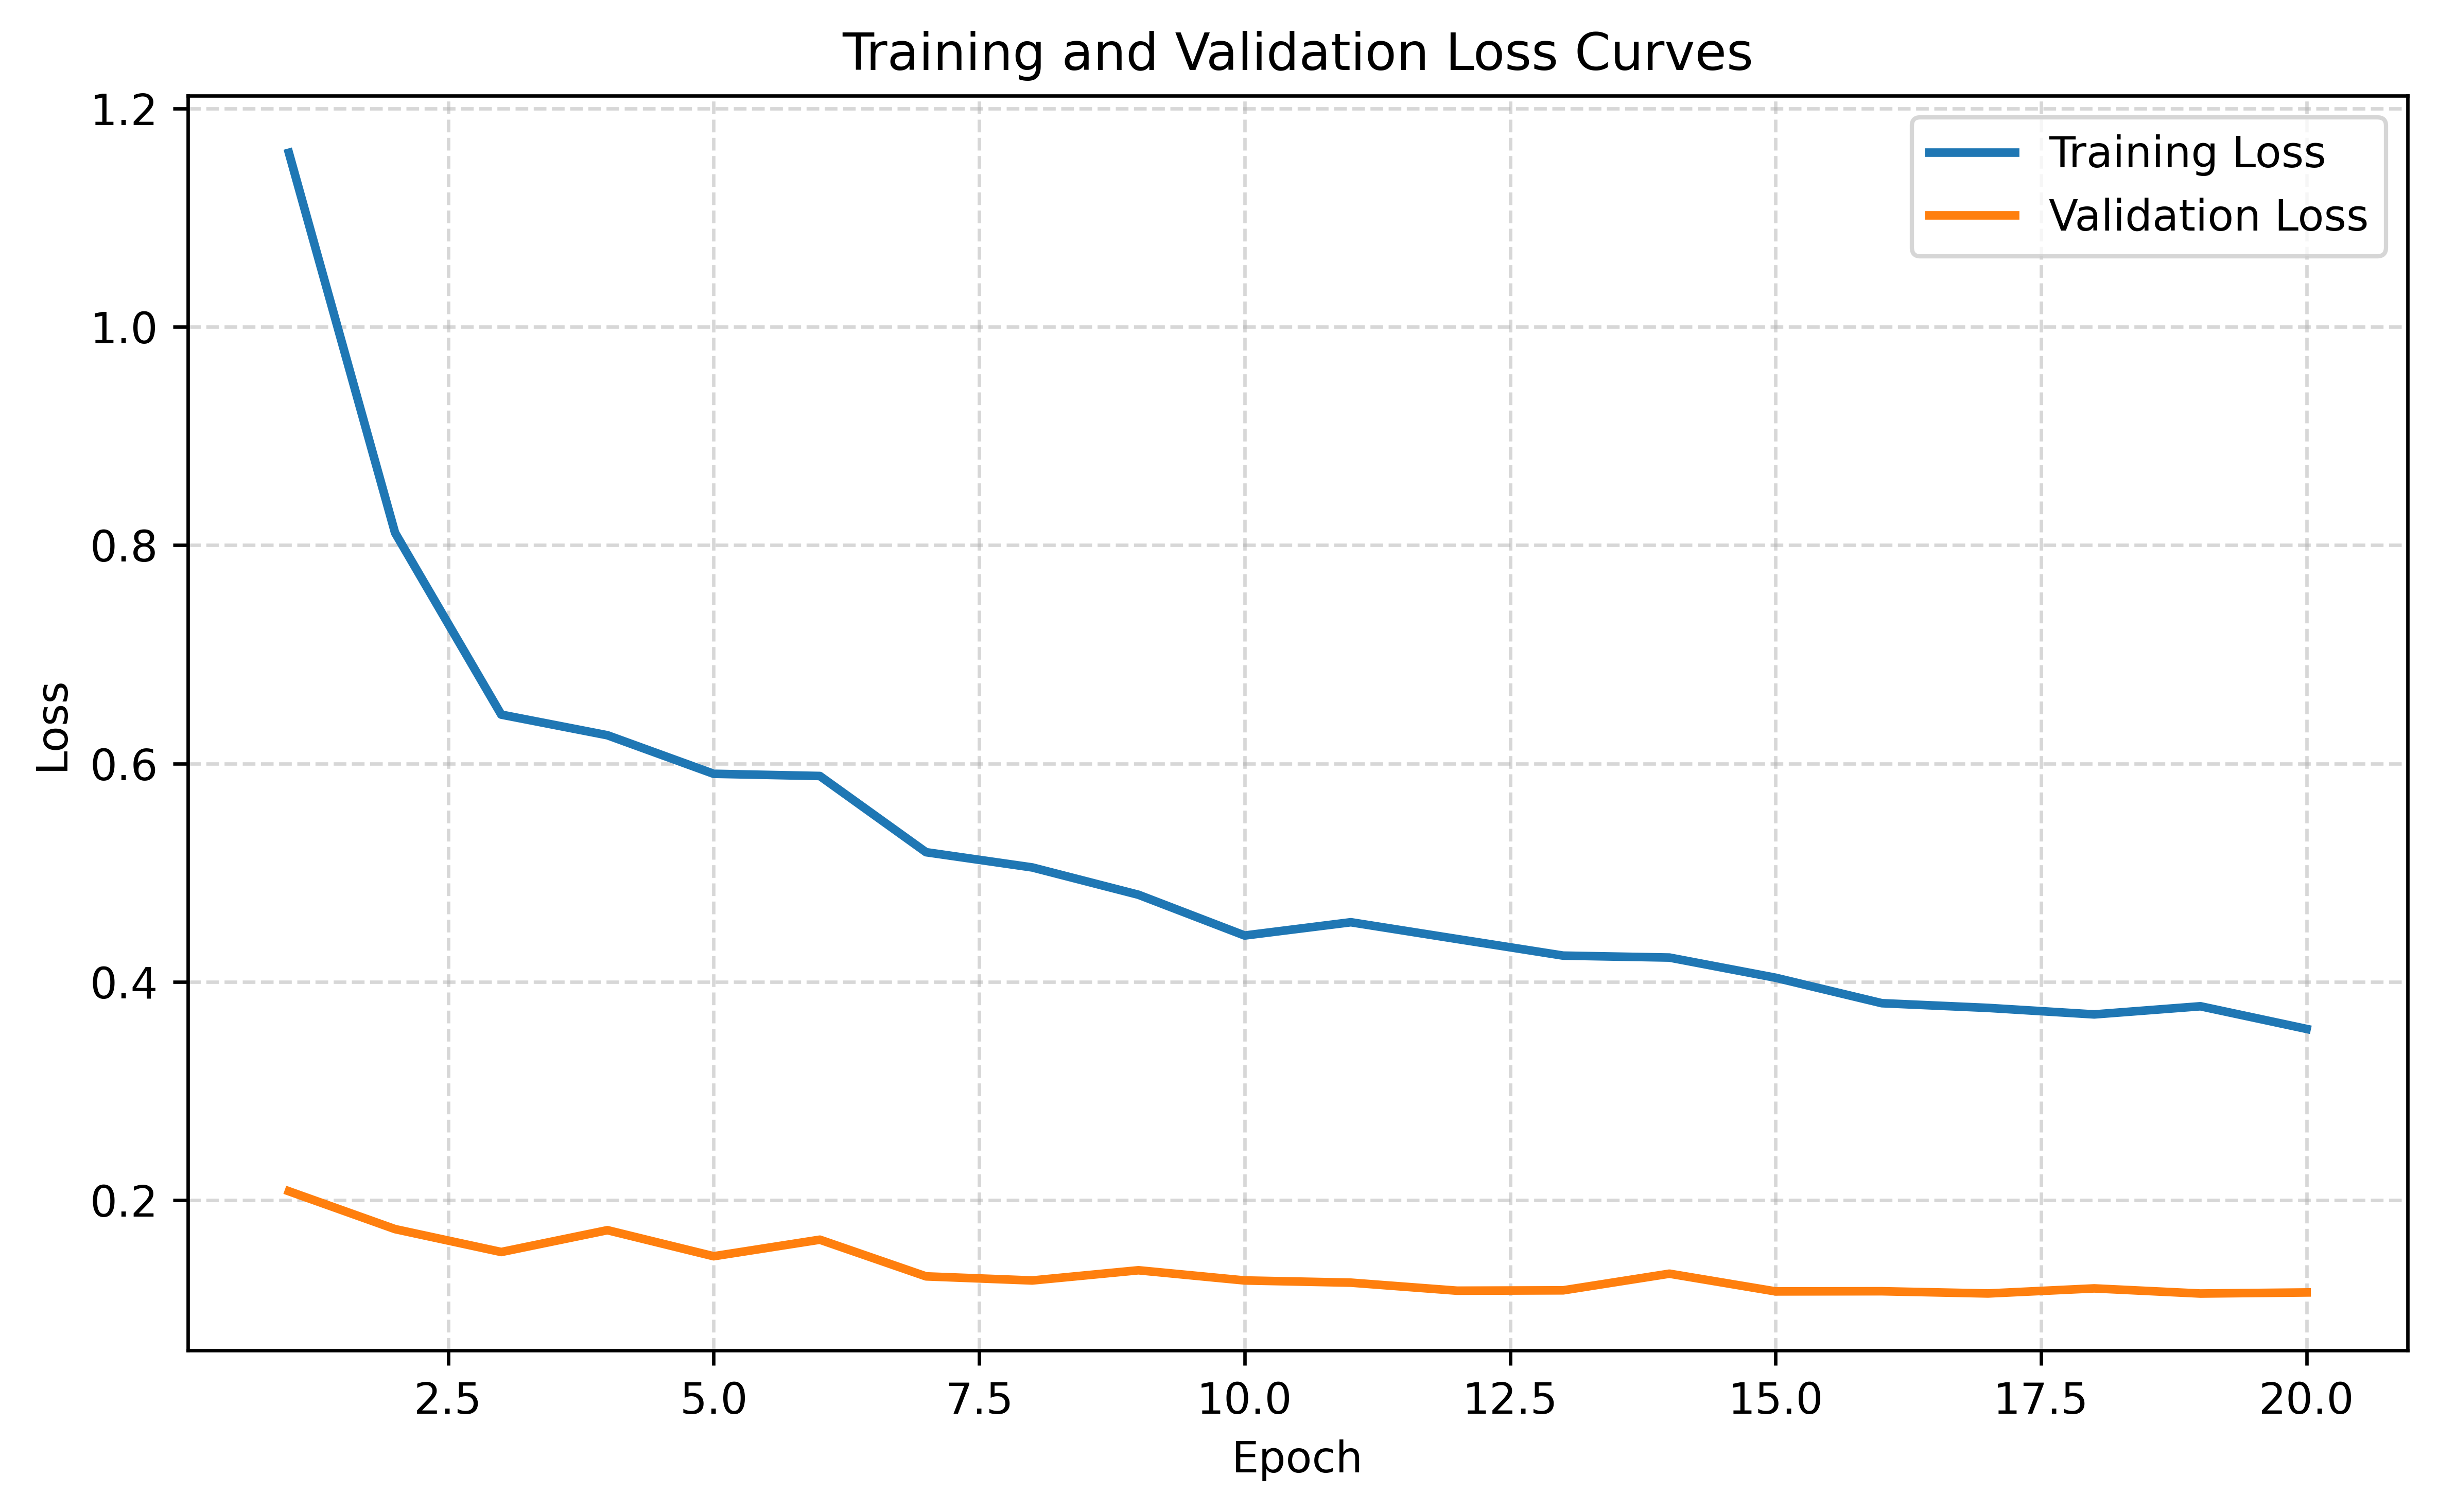
\includegraphics[width=\linewidth]{Images/loss_curves (1).png}
\caption{Training and validation losses.}
    \label{fig:loss_curves}
\end{subfigure}
\hfill
\begin{subfigure}[t]{0.48\textwidth}
    \centering
    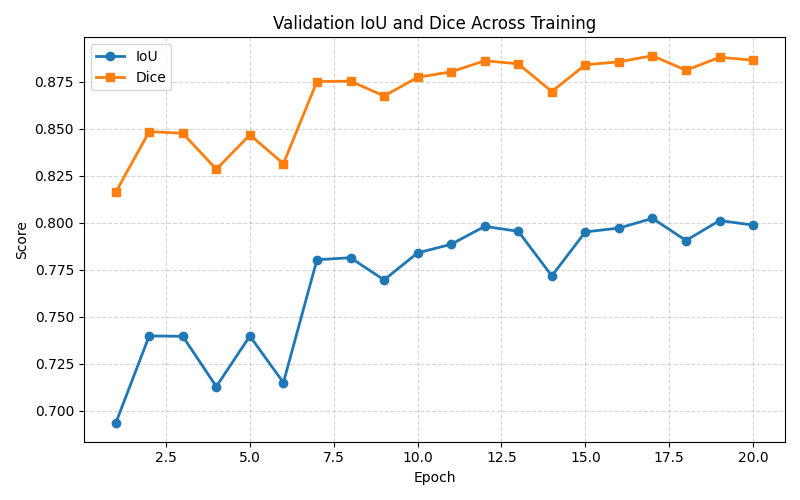
\includegraphics[width=\linewidth]{Images/ioudice_new.png}
\caption{Validation IoU and Dice scores.}
    \label{fig:iou_dice}
\end{subfigure}

\caption{Training dynamics of $M^2$FA-Net
over 20 epochs.}
\label{fig:training_dynamics}

\end{figure*}

\section{Conclusion and Future scope}
\label{sec:limitations}

In this paper, we proposed $M^2$FA-Net, a multimodal fusion framework for crop--weed segmentation that integrates dual-stream DeepLabV3 backbones, multi-level feature fusion, CBAM attention, deep supervision, and a composite loss function. The proposed framework effectively combines spatial, spectral, and vegetation-index information, achieving 80.79\% IoU and 89.21\% Dice score on the WeedyRice-RGBMS-DB dataset, outperforming the evaluated baseline models. These results demonstrate the effectiveness of $M^2$FA-Net on the evaluated benchmark. Input-modality ablation further indicates a modest but consistent improvement from multispectral bands, while NDVI and NDRE provide no clear additional benefit.


This work has several limitations. Experiments were conducted on a single dataset of 734 samples collected using one sensor in An Giang, Vietnam, with the image-level split provided by the dataset authors. Although the images were acquired across multiple cropping seasons, the documentation does not confirm whether the partitions are independent by field, UAV flight, or acquisition date. Consequently, spatially or temporally adjacent images may occur across training and test partitions, potentially leading to optimistic performance estimates. The reported results therefore primarily reflect generalization within this dataset. Furthermore, the modest contribution of multispectral bands and vegetation indices may vary across crops, growth stages, and sensors. The model's computational requirements and lack of edge-device evaluation also limit conclusions about real-time onboard UAV deployment.

Future work will focus on improving generalization, computational efficiency, and practical deployment. Few-shot learning, domain adaptation, domain generalization, and self-supervised multimodal pretraining may improve performance across different agricultural conditions while reducing annotation requirements. Lightweight variants will be explored for deployment on UAVs and edge devices, along with extensions to multi-class segmentation and spatiotemporal analysis. Independent cross-field, cross-season, and external-dataset evaluations will also be conducted to assess generalization more rigorously.

\section*{Author Contributions}

Manan Dudeja: Methodology, Software, Data curation, Validation, Writing--original draft.
Rakesh Kumar Sanodiya: Origination and Conceptualization, Data curation, Validation, Supervision, Project administration, Investigation, Writing--review \& editing.
Lekshmi R: Formal analysis, Visualization, Investigation.
Matloob Khushi: Conceptualization, Validation, Supervision, Project administration, Writing--review \& editing.

\section*{Acknowledgment}
We thank the anonymous reviewers for their careful reading and constructive feedback, which helped improve this manuscript.

\section*{Funding}
This work was supported by the
Science and Engineering Research Board (SERB)
under the Core Research Grant Project (File No. 
CRG/2023/001239). 

\section*{Data Availability}

The WeedyRice-RGBMS-DB dataset used in this work is publicly available at: 

https://data.mendeley.com/datasets/vt4s83pxx6/1

\section*{Competing Interests}

The authors declare that they have no competing interests.


\bibliography{sn-bibliography}



\end{document}